% This is samplepaper.tex, a sample chapter demonstrating the
% LLNCS macro package for Springer Computer Science proceedings;
% Version 2.20 of 2017/10/04
%
\documentclass[runningheads]{llncs}
%
\usepackage{graphicx}
\usepackage{tikz}
\usepackage{subcaption}
\captionsetup{compatibility=false}
\newcommand*\rot{\rotatebox{90}}
\usepackage{amssymb}
\usetikzlibrary{positioning}

\usetikzlibrary{arrows}

\usepackage{amsmath}
\usepackage{booktabs}
\usepackage[ruled,noend,vlined,linesnumbered]{algorithm2e}

% Used for displaying a sample figure. If possible, figure files should
% be included in EPS format.
%
% If you use the hyperref package, please uncomment the following line
% to display URLs in blue roman font according to Springer's eBook style:
% \renewcommand\UrlFont{\color{blue}\rmfamily}
\usepackage{color}


\input{draft_tools}
\input{commands}


\begin{document}
%
\title{Rule Induction and Reasoning over Knowledge Graphs}
%
%\titlerunning{Abbreviated paper title}
% If the paper title is too long for the running head, you can set
% an abbreviated paper title here
%
\author{First Author\inst{1} \and
Second Author\inst{1} \and
Third Author\inst{1}}


%
\authorrunning{F. Author et al.}
% First names are abbreviated in the running head.
% If there are more than two authors, 'et al.' is used.
%
\institute{Max Planck Institute for Informatics,\\ Saarland Informatics Campus, Germany\\
\email{lncs@springer.com}\\
%\url{http://www.springer.com/gp/computer-science/lncs} \and
%ABC Institute, Rupert-Karls-University Heidelberg, Heidelberg, Germany\\
%\email{\{abc,lncs\}@uni-heidelberg.de}
}
%
\maketitle              % typeset the header of the contribution
%
\begin{abstract}
Advances in information extraction have enabled the automatic
construction of large knowledge graphs (KGs) like DBpedia, Freebase, YAGO
and Wikidata. Learning rules from KGs is a crucial task for KG completion,
cleaning and curation. This tutorial presents state-of-the-art rule
induction methods, recent advances, research opportunities as well as open
challenges along this avenue. We put a particular emphasis on the problems
of learning exception-enriched rules from highly biased and incomplete
data. Finally, we discuss possible extensions of classical rule induction
techniques to account for unstructured resources (e.g., text) along with
the structured ones.
%\keywords{First keyword  \and Second keyword \and Another keyword.}
\end{abstract}



\section{Introduction}
\label{sec:intro}

\begin{itemize}
\item
\end{itemize}
\section{Knowledge Graphs}
\label{sec:kgs}

% \subsection{Graph-based Representation}
Knowledge Graphs (KGs) have been introduced in the Semantic Web community to create the ``Web of data" that can be readable by machines. They represent interlinked collections of factual information, which are often encoded using the RDF data model \cite{rdf2004}. This data model represents the content of the graph with a set of triples of the form $\tuple{\mi{subject\;predicate\;object}}$ corresponding to positive binary and unary first-order logic (FOL) facts. For encyclopedic KGs on the semantic web, usually the open world assumption (OWA) is employed, i.e., these graphs contain only a subset of the true information. % are large collections of information modeled in the form of entities (such as people, organizations, or places) and the relationships between them.
%KGs %were 
%is
%can be . % This was pushed forward by introducing the W3C Resource Description Framework (RDF)~\cite{rdf2004}.
%Under this representation, the entities are encoded as the nodes of the graph and the relations as directed edges between them
%~\cite{Nickel2015ARO}. 
%In various literature, for simplicity KGs are represented as sets of triples in the form of $\tuple{subject, predicate, object}$ (SPO triples, for short). Alternatively, others adopt a factual representation for which a KG $\cG$ is defined over the signature $\Sigma_{\cG}=\tuple{\cR,\cC}$, where $\cR$ is the set of binary predicates (aka relations) and $\cC$  is the set of constants (aka entities) appearing in $\cG$.  
%\gad{could you please check this KG signature def?}\ds{please fix typos, otherwise it is ok}

\begin{example} Figure~\ref{rdf} shows a snippet of a graph about people, marriage %their 
relations between them %to each other and 
their %places of 
living places. For instance, the upper half encodes the information that ``Ann has bother john, and lives with her husband Brad in Berlin, which is a metropolitan.''. 
%while her brother John lives in Chicago with his wife Kate. Moreover, both Berlin and Chicago are metropolitans'', which %would also 
is % also 
represented as the set of FOL facts $\mi{\{hasBrother(ann, john), livesIn(ann, berlin)}$, $\mi{livesIn(brad, berlin)}$,\\ $\mi{isMarriedTo(brad, ann)}$
% $\mi{hasBrother(ann, john)}$, \\$\mi{livesIn(john, chicago)}$, $\mi{livesIn(kate, chicago)} \}$, $\mi{isMarriedTo(john, kate)}$,
$\mi{metropolitan(berlin)}\}$.  \qed
\end{example}
%\begin{example}
%The statement \textit{``Christopher Nolan is the director of the science fiction movie Interstellar, which won the Best Visual Effects Oscar"} will be represented in several SPO triples:\\
%$\tuple{chris\_nolan, isA, director}$,\\
%$\tuple{chris\_nolan, directed, interstellar}$,\\
%$\tuple{interstellar, gerne, science\_fiction}$, and \\
%$\tuple{interstellar, wonPrize, visual\_effects\_oscar}$.
%\end{example}





%about people, organizations, places, etc. Predicates encodes the relations between them, \eg $\tuple{einstein, wasBornIn, Ulm}$. KGs can also be represented similar to formal logic syntax as binary predicate $p(s,o)$, where $subject$ and $object$ are the arguments. KGs can be seen as instantiations for some ontological schema.  
%\leanparagraph{Definition}

\subsection{Knowledge Graphs Construction and Quality}
% Please add the following required packages to your document preamble:
% \usepackage{booktabs}
\begin{table}[t]
\centering

\label{tab:kgs}
\begin{tabular}{@{}llll@{}}
\toprule
Knowledge Graphs       & \# Entities & \# Relations & \# Facts \\ \midrule
DBpedia                &             &              &          \\
Freebase               &     40 M    &      35000   &    637 M \\
YAGO3                  &             &              &          \\
Wikidata               &             &              &          \\
WordNet                &             &              &          \\
Google Knowledge Graph &      570 M  &       35000  &   18000 M\\ \bottomrule
\end{tabular}
\caption{Example real life knowledge graphs and their sizes}

\end{table}
KGs are constructed either manually or automatically. Manually constructed KGs are either curated by a closed group of experts, %as for 
e.g., WordNet~\cite{wordnet} or collaboratively by volunteers, 
%such as 
e.g., Freebase~\cite{Freebase} and Wikidata~\cite{wikidata}.  Nevertheless, there is extensive work for automatically populating KGs from semi-structured resources such as Wikipedia info-boxes using regular expressions and other heuristics and constraints as in YAGO~\cite{yago} and DBpedia~\cite{dbpedia}. More eager approaches propose extracting facts from unstructured resources using natural language processing and machine learning techniques; resulting in KGs such as  NELL~\cite{nell}, KnowledgeVault~\cite{KnowledgeVault}. Table~\ref{tab:kgs}, shows examples for several available KGs (extended discussions can be found in~\cite{Nickel2015ARO,DBLP:journals/semweb/Paulheim17}). 

%\gad{should we speak about the sizes and scalability of existing approaches}\ds{reporting statistics is enough}


Both manually and automatically constructed KGs are still far from modeling the real world in two aspects: (i) they are still \textit{incomplete} with relatively \textit{low coverage} for the existing real-world entities and the possible inter-entities relationships. (ii) they have \textit{inaccurate} facts resulting from the extraction errors and the heuristic methods applied while construction as well.  



\subsection{Interpreting Knowledge Graphs under Incompleteness}

Existing KGs consist of positive facts only (\ie true relations). There are two paradigms to interpret the missing fact: (i) under \textit{closed world assumption} (CWA), in which missing edges indicate a false relationship. (ii) under open world assumption (OWA), such that non-existing relations are interpreted as unknown and can be either true or false. For example, in Figure~\ref{rdf}, the missing \textit{livesIn} link between \textit{Dave} and \textit{Chicago} would be interpreted as $\neg livesIn(dave, chicago)$ under CWA. However, under OWA, no conclusion can be made. Given the \textit{incompleteness} and \textit{inaccuracy} of the existing real-life KGs, they are usually interpreted under OWA~\cite{Nickel2015ARO}. 

To study the incompleteness of KGs, we assume the existence of an ideal graph $\cG^i$ containing a snapshot of the current world; hence, we define the incompleteness of knowledge graphs as:

\begin{definition}[Incomplete Knowledge Graph] An incomplete KG is a pair
    $G = (\cG, \cG^i)$ of two KGs, where $\cG\subseteq \cG^i$ and
    $\Sigma_{\cG}=\Sigma_{\cG^i}$. We call $\cG$ the available
    graph and $\mathcal{G}^i$ the ideal graph.  \end{definition}
    
This definition allows evaluating the proposed approaches for completing the knowledge graph.  


\section{Reasoning over Knowledge Graphs (1.5 pages)}
\label{sec:reasoning}

\leanparagraph{Rules}

\leanparagraph{Types of Rules}

\leanparagraph{Applying rules on KGs}


\section{ Rule Learning for Knowledge Graph Completion}
\label{sec:rules_kg_completion}
In this section we first describe the possible learning tasks that could be performed over KGs and then dwell into the details of the relational association rule learning from incomplete KGs. 
\subsection{Rule Learning Tasks}
\label{sec:rules_learning_tasks}
Rule learning is an important sub-field of machine learning research area, which focuses on symbolic methods for intelligent data analysis. Hereby symbolic, we mean methods that employ some kind of description language in which the learned knowledge is expressed. One of the main attractions of rule induction is that the rules are much more transparent and easier to interpret than, e.g., a regression model or trained neural network.

First-order learning approaches are also referred to as %\emph{relational data mining (RDM)}, \emph{relational learning
%(RL)} or
 \emph{inductive logic programming (ILP)}, since the patterns they discover are expressed in
relational formalisms of first-order logic (see \cite{DBLP:books/daglib/0021868} for overview).

Rule learning approaches can be characterized along several dimensions \cite{DBLP:conf/semweb/SazonauS17}: 
\begin{itemize}
\item \emph{type of the data source}, e.g., KG, database, text, oracle (a domain expert), true and false facts over a certain target predicate (often referred to as positive and negative examples respectively)
\item \emph{type of the output knowledge}, e.g., Horn rules, description logic class descriptions, class inclusions of various expressivity, etc.
\item \emph{method used}, e.g., natural language processing, machine learning, association rule mining, theory revision, oracle-based exact learning techniques, etc.
\item \emph{data (in)completeness assumption}, e.g., OWA, CWA, partial completeness assumption, etc.
\item \emph{availability and type of background knowledge}, e.g., DL ontology, set of datalog rules.
\end{itemize}

The most prominent setting that has been extensively studied in the context of inductive logic programming concerns the extraction of a hypothesis in a certain language, given a set of positive and negative examples and a logical background theory in the form of a logic program, e.g., \cite{foil,golem,quickfoil}. To get an idea of this classical ILP task, consider the following example.

\begin{example}
Suppose that you possess information about some of the relationships between people in your family and their genders.
However, you do not know what the relationship $\mi{fatherOf}$ actually means. 
You might have the following beliefs, i.e., background knowledge.
\smallskip

{\leftline{$B = \left\{
            \renewcommand{\arraystretch}{1.1}
            \begin{array}{@{\,}l@{~~}l@{}}
              \mbox{(1) } \mi{parent (john, mary)};
               \mbox{(2) }\mi{male(john)};
              \mbox{(3) }\mi{parent (david, steve)};\\
              \mbox{(4) }\mi{ male(david)};
              \mbox{(5) }\mi{parent (kathy, ellen)};
              \mbox{(6) }\mi{ female (kathy)};
            \end{array}%
            \!\right\}$}}
\smallskip

Moreover, you are given the following positive and negative examples.
\smallskip

\noindent $\mi{E^+=\{fatherOf(john, mary), fatherOf(david, steve)\}}$\\
$\mi{E^-=\{fatherOf(kathy, ellen), fatherOf(john, steve)\}}$\\



One of the possible hypothesis that can be induced from the above knowledge reflecting the meaning of the $\mi{fatherOf}$ relation is given as follows:\\
$\mi{Hyp: fatherOf(X, Y)\leftarrow parentOf(X,Y), male(X)}$. This hypothesis is consistent with the background theory $B$, and together with B it entails all of the positive example, none of the negative ones, i.e., $\mi{Hyp \cup B \models B^+}$ and $\mi{H \cup B \not \models E^-}$. The classical ILP task concerns the extraction of such hypothesis. \qed
\end{example}

While a significant amount of research has been devoted to the problem of inducing logical theories from a set of positive and negative examples and the background knowledge (as exemplified above), there are several important obstacles that prevent one from employing the off-the-shelf ILP algorithms for solving the rule-based KG completion problem from Definition~\ref{def:kgcomp}. 

First, the target predicates ($\mi{fatherOf}$ from the above example) can
not be easily identified, since we do not know which parts of the considered KG need to
 be completed. A standard way of addressing this issue would be just to learn rules for all
 the different predicate names occurring in the KG. Unfortunately, this is unfeasible
 given the huge size of KGs. Second, the negative examples are not available,
 and they can not be easily obtained from, e.g., domain experts due to - once again
 - the huge size of KGs. % A natural solution to cope with this issue is to learn rules
% from positive examples only \cite{DBLP:conf/ilp/Muggleton96}. 

To overcome the above obstacles, it turns out to be appropriate to treat
the KG completion problem as an unsupervised relational learning task \cite{amie}.
In fact, association rules in their original propositional form have been earlier applied to deduce missing types for entities in \cite{typeinduction} and to
infer the KG schema in \cite{statisticalschema}. These works directly employ the famous Apriori algorithm for mining frequent itemsets from transaction databases.
%Third, the definition of a language bias turns out to be
% cumbersome since the schema of the KG is usually not available.

In the rest of this section, we describe approaches that rely on \emph{relational association rule learning} techniques for extraction of \emph{Horn rules} from incomplete KGs. 
Association rule mining concerns the discovery of frequent patterns in a data set and the subsequent transformation of these patterns into rules
(see, e.g., \cite{DBLP:conf/ilp/DehaspeR97} as the seminal work in this direction). % In the following we adapt basic notions in relational association rule mining to our case of interest.

The standard relational rule learning techniques usually proceed in two 
steps: rule construction and rule evaluation. While the main concern of the rule construction phase is how to mine frequent patterns from the KG, 
%and transform them into the form of rules, 
rule evaluation phase deals with measuring rule quality %from 
using some scoring function computed based on the rule statistics over the given KG. These statistics are used not only for ranking the outputting rules, but also for pruning inappropriate rule candidates. Below, we summarize some general techniques that have been introduced to tackle the mentioned rule learning steps.

\subsection{Rule Construction}
% Traditional rules learning systems in the context of Inductive Logic Programming (ILP) \cite{probfoil,DBLP:conf/ijcai/RaedtDTBV15,DBLP:conf/clima/CorapiSIR11} are either memory-expensive or requires the availability of negative examples, which is hard to get due to the large KG size. In contrast, other unsupervised relational 
% association rule learning systems deduce logical rules from the KG by mining frequent patterns and casting them into implications. Most of the  existing methods tailored towards Open World Assumption (OWA) rely only on the available graph and exploit sophisticated rule measures \cite{amie,op,rumis}.

We now briefly summarize some of the state-of-the-art methods %rule mining systems, 
for rule construction, most of which % which combine rule learning and reasoning for knowledge graph completion under OWA.
%Most of these systems only 
extract so-called \emph{closed} rules,
i.e., rules, in which every variable appears at least twice. Restriction to closed rules % is imposed to 
ensures the actual prediction  of a fact by a rule, but not just its existence~\cite{amie}.

\begin{example}
%\ds{TODO: insert an example of a closed and a non-closed rule, say a few words, why closed rules make sense}
An example of non-closed rule learned from the KG in Figure~\ref{rdf} is % , a non-closed rule learned from this graph can be:
\[\exists Z \mi{livesIn(Y,Z)} \leftarrow \mi{isMarriedTo(X,Y)} \]  which states that married people 
%then he/she should 
live in some place. Unlike $r_1$, this rule cannot infer the exact living place of a person of interest is thus less interesting. \qed% for the KG completion. %location 
%which specifies his living location based on the spouse.
\end{example}

The most prominent examples of systems that are specifically tailored towards inducing rules from KGs are AMIE \cite{amie}, %OP, \cite{op} 
and RDF2Rules \cite{rdf2rules}.
\subsubsection{AMIE.}
AMIE \cite{amie} is a state-of-the-art Horn rule mining system.
Apart from a KG, it expects from the user a support threshold and maximum
rule length. The algorithm maintains a queue of rules, which initially stores a single rule with an empty body for every KG relation. 
Rules are removed from the queue and refined by adding literals to the body according to a language bias that specifies allowed rule forms (e.g., based on the user-provided rule length). The system then estimates the support of the rule, and if it exceeds the given threshold, the rule is output to the user and also added to the queue for
possible further processing.
%Apart from the algorithm being used to construct rules, AMIE also introduces a novel rule measure namely PCA confidence, which is based on the Partial Closed world Assumption (PCA), stating that data of the knowledge graph is added in batch \cite{amie}. In particular, with every $p(s,o) \in \cG$, the assumption states that:
%\[\forall o' : p(s,o') \in \cG^i \Rightarrow p(s,o') \in \cG\]
%Intuitively, if the KG contains some $p$-object of $s$, then it also contains all possible $p$-objects of $s$. Formally, PCA confidence is defined as follows:\thi{pca conf here}
%\[conf_{pca}=.\]
%This measure is then exploited by AMIE to mine positive rules using its introduced algorithm. 
Refinement of a rule relies on the following set of mining operators used to extend the sequences of atoms in the rule body:
\begin{itemize}
\item \textit{add dangling atom}: add a new positive atom with one fresh variable, i.e., variable not appearing elsewhere in the rule;
\item \textit{add instantiated atom}: add a positive atom with one argument being a constant and the other one being a shared variable, i.e., variable already present in another rule atom;
\item \textit{add closing atom}:  add a positive atom with both of its arguments being shared variables.

\end{itemize}
%\begin{algorithm}[t]
%\DontPrintSemicolon
%$queue\leftarrow \langle[]\rangle$\\
%Execute in parallel:\\
%\While{$\neg$queue.isEmpty()}{    
%    \textit{rule $\leftarrow$ queue.dequeue()}\\
%%    \tcc{Computes rule statistics and output if necessary.}
%    \If{rule.isClosed()}{
%        \eIf{rule is not pruned for outputting}{
%            output($rule$)
%        }{
%            continue while loop
%        }
%    }
%%    \tcc{Applies operators to explore more new rules.}
%    \ForEach{operator o}{
%        \ForEach{newRule $\in$ o(rule)}{
%%            \If{newRule.hasGoodFormat()}{
%%                \tcc{Check whether there exists some version of the rule in queue.}
%                \If{newRule $\notin$ queue}{ 
%                    \textit{queue.enqueue(newRule)}
%%               }
%            }
%        }
%    }    
%}
%\caption{AMIE's mining algorithm.}
%\label{algor:amie}
%\end{algorithm}
% These mining operators are then applied to extract rules from KGs. The algorithm maintains a queue consisting of intermediate rules to be processed. At the beginning, the queue contains only an empty rule. At each step, one rule is taken from the head of the queue, then being checked for outputting. Then, mining operators are applied to explore new more rules.
% Checking for outputting is the process of collecting rule statistics (e.g. \textit{support}, \textit{confidence}), and then checking whether these metrics pass some defined threshold. Apart from that, the expansion of rules must meet the other two requirements: the increasing of rule quality, and the language bias. In particular, firstly, adding an atom into the rule must increase its quality (e.g. \textit{confidence}). Secondly, the rules being outputted must be \textit{closed} and number of atoms of the rule does not exceed some threshold.

% To compute the rule's statistics, we must find all instantiations of variables in a rule in the given KG. Several options have been proposed depending on how the KGs are stored: either by using SQL, SPARQL or using in-memory database techniques \cite{amie}.
The implementation of AMIE employs a variety of techniques from the database community, which allow it to achieve high scalability.

\subsubsection{RDF2Rules.}
While AMIE mines one rule at a time, RDF2Rules \cite{rdf2rules} parallelizes this process by extracting \emph{frequent predicate cycles} (FPCs) of %some 
a certain length $k$, which have the following form:
\[\theta = (X_1, p_1^{d_1}, X_2, p_2^{d_2},\dotsc, X_k, p_k^{d_k}, X_1)\]
where, $X_i$s are variables to appear in the rules, $p_i$s are predicates between these variables, and $d_i$s $\in \{0,1\}$ reflect the direction of the edges in the KG labeled by the respective predicates. To extract FPCs, the algorithm first mines the \emph{frequent predicate paths} (FPPs) of the form:
\[\theta = (X_1, p_1^{d_1}, X_2, p_2^{d_2}, ...,X_k, p_k^{d_k}, X_{k+1})\]
of length $k$, which could be mined recursively based on FPPs of length $k-1$. 
FPCs are then created from FPPs by merging the last variable $X_{k+1}$ with the first one $X_1$.

After mining FPCs, rules are extracted from the FPCs by choosing one %a 
predicate to be in    %as 
the head, and collecting the rest into the rule's  body. 
%of the rule. 
Formally, the  $j$-th rule is generated from the FPC as follows:
\[r_j: p_j^{d_j}(X_j,X_{j+1}) \leftarrow \underset{i \in [1,k], i \ne j}{\bigwedge} p_i^{d_i}(X_i,X_{i+1}) \]

RDF2Rules is capable of accounting for unary predicates (i.e., types of entities), which are neglected in AMIE for scalability reasons. % The above generated rules are without \textit{type} information.
The unary predicates are added to the constructed rule at the last stage after analyzing the 
frequent types for FPCs corresponding to a given rule.
% Nevertheless, comparing to AMIE, even though RDF2Rules can mine rules faster, the forms of rule it can learn are restricted, s
While RDF2Rules performs the rule extraction faster then AMIE due to an effective pruning strategy
used in the process of mining FPCs, the supported rule patterns are also more restrictive. 

\subsection{Rule Evaluation}
Most of state-of-the-art KG-based positive rule mining systems %are different 
differ from each other with respect to the employed %at the rule %metric 
%that they introduce to quantify 
rule ranking function. % quality and how to exploit it in learning rules. 
%Basically, we can plug different rule metrics into these mining systems to work under different situations.
The ranking metrics from datamining such as support and confidence (see, e.g., \cite{metrics-summary} for overview of others) presented in Section~\ref{sec:reasoning} have been designed for datasets that operate primarily under the CWA, and they can be counterintuitive for the KGs, in which facts are largely missing. 

\begin{example}
For instance, consider a KG $\cG'$ in Figure~\ref{fig:fam_grad} \cite{carl}, which presents information about scientific families.
The heavily biased rule from Section~\ref{sec:intro}: $\mi{r_1':\;hasChild(X,Y)\leftarrow worksAt(X,Z), educated(Y,Z)}$ can be mined from it along with a good one $\mi{r_2':\,hasSibling(X,Z)\leftarrow hasFather(X,Y),hasChild(Y,Z)}$, stating that people with the same father are likely siblings. The standard rule measures such as confidence reflect a counterintuitive rule preference. Indeed, we have $\mi{conf(\mi{r_1'})}=\frac{2}{8}$, while
 %we have that 
$\mi{conf(\mi{r_2'})}=\frac{1}{6}$. \qed
\end{example}

 % For instance, standard confidence $conf$ works under the Closed World Assumption.
% Apart from that, there also exist other measures introduced to quantify the quality of rules (see
%). 
 \begin{figure}[t]
\centering
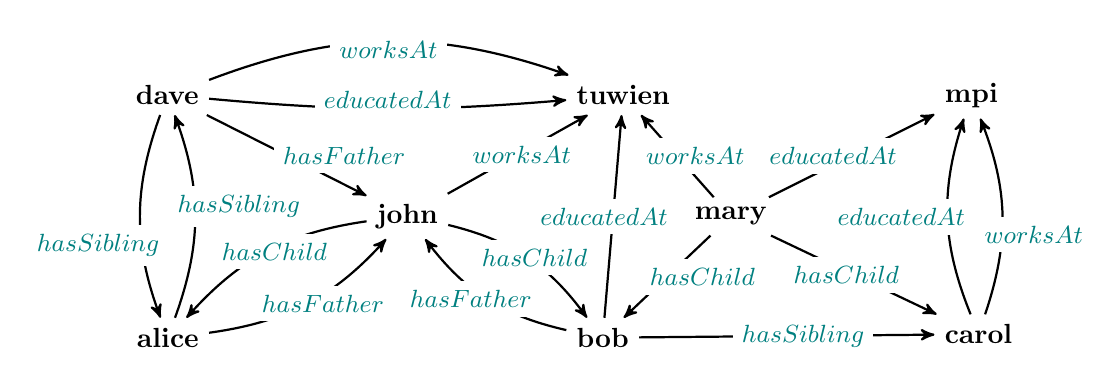
\begin{tikzpicture}[->,>=stealth',auto,node distance=3cm,
  thick,main node/.style={font=\bfseries}]

  \node[main node] (1) {john};
  \node[main node] (2) [right=3cm of 1] {mary};
  \node[main node] (3) [below left=1cm and 2cm of 1] {alice};
  \node[main node] (4) [below right=1cm and 1.5cm of 1] {bob};
  \node[main node] (5) [below right=1cm and 2cm of 2] {carol};
  \node[main node] (6) [above left=1cm and 2cm of 1] {dave};
  \node[main node] (7) [above right=1cm and 1.5cm of 1] {tuwien};
  \node[main node] (8) [above right=1cm and 2cm of 2] {mpi};

  \path[every node/.style={color=teal,fill=white,font=\small}]
    (1) edge node [right=-20pt] {$\mi{worksAt}$} (7)
    (2) edge node [right=-15pt] {$\mi{worksAt}$} (7)
    (4) edge node [right=-30pt] {$\mi{educatedAt}$} (7)
    (2) edge node [right=-10pt] {$\mi{hasChild}$} (4)
    (2) edge node [left=-20pt] {$\mi{hasChild}$} (5)
    (1) edge[bend left=20] node [right=-20pt] {$\mi{hasChild}$} (4)
    (4) edge[bend left=20] node [left=-20pt] {$\mi{hasFather}$} (1)
    (1) edge[bend right=20] node [right=-20pt] {$\mi{hasChild}$} (3)
    (3) edge[bend right=20] node [right=-20pt] {$\mi{hasFather}$} (1)
    (2) edge node [left=-20pt] {$\mi{educatedAt}$} (8)
    (5) edge[bend left=20] node [left=-10pt] {$\mi{educatedAt}$} (8)
    (5) edge[bend right=20] node [right=-10pt,pos=0.4] {$\mi{worksAt}$} (8)
    (6) edge node [right=-5pt] {$\mi{hasFather}$} (1)
    (3) edge[bend right=20] node [right=-10pt,pos=0.55] {$\mi{hasSibling}$} (6)
    (6) edge[bend right=20] node [left=-10pt,pos=0.65] {$\mi{hasSibling}$} (3)
    (6) edge[bend left=20] node [above=-10pt] {$\mi{worksAt}$} (7)
    (6) edge[bend right=5] node [below=-10pt] {$\mi{educatedAt}$} (7)
    (4) edge node [right=-20pt] {$\mi{hasSibling}$} (5)
    ;
\end{tikzpicture}
\caption{Example KG: family relations, working and education places.}
\label{fig:fam_grad}
\end{figure}
% Given $r:\mi{H\leftarrow B, \naf\ E}$, with $H=\mi{h(X,Y)}$ and $B,E$ involving variables from $\vec{Z}\supseteq X,Y$, and also consider the example rules $r_1$, $r_2$, KG $\cG_1$ in Figure \ref{rdf}, we have:
\subsubsection{PCA Confidence.} Proposed by AMIE \cite{amie}, this measure considers KGs under the Partial Completeness Assumption (PCA), saying that data of the knowledge graph is added in batch \cite{amie}. In particular, with every $p(s,o) \in \cG$, the assumption states that:
\[\forall o' : p(s,o') \in \cG^i \implies p(s,o') \in \cG\]
Intuitively, if the KG contains some $p$-object of $s$, then it also contains all possible $p$-objects of $s$. Formally, \textit{PCA confidence} is defined as follows:
\[
\mi{conf_{pca}}(r, \cG) := \frac{\textit{r-supp}(r, \cG)}{\#(X,Y): \exists \vec{Z}: B \in \cG, E \notin \cG  \wedge \exists Y': h(X,Y')\in \cG}
\]
\begin{example}
We have $conf_{pca}(r_1,\cG_1) = \frac{3}{4}$, since we do not know any place where $lucy$ and $dave$ live. Similarly, $conf_{pca}(r_2),\cG_1) = \frac{3}{3}$.\qed
\end{example}
\subsubsection{Conviction.} \textit{Conviction} is shown to guarantee the high predictive power \cite{Azevedo2007} by measuring the intensity of rule's implication \cite{metrics-summary}, which is given by:
\begin{align*}
\textit{conv}(r,\cG) & := \frac{1 - \textit{rel-supp}(H, \cG)}{1-\textit{conf}(r,\cG)}
\end{align*}
where $\textit{rel-supp}(H, \cG)$ is the relative support of the head, measured by:
\begin{align*}
\textit{rel-supp}(H, \cG) = \dfrac{\#(X,Y):h(X,Y)\in \cG}{(\#X:\exists Y:h(X,Y)\in \cG)\times(\#Y:\exists X:h(X,Y)\in \cG)}
\end{align*}
\begin{example}
We have $\textit{rel-supp}(livesIn, \cG_1) = \frac{10}{10 \times 4} = \frac{1}{4}$, so $conv(r_1,\cG_1) = \frac{1-\frac{1}{4}}{1-\frac{3}{6}} = \frac{3}{2}$ and $conv(r_2,\cG_1) = \frac{1-\frac{1}{4}}{1-\frac{3}{4}} = 3$.\qed
\end{example}
\subsubsection{Soft Confidence.} Introduced by RDF2Rules \cite{rdf2rules}, \textit{soft confidence} is also tailored to work under Open World Assumption, measured by:
\[conf_{st}(r, \cG) = \frac{\textit{r-supp}(r, \cG)}{\textit{b-supp}(r,\cG) - \sum_{e \in U_r}P(e,p,\cG)} \]
where $U_r$ is the set of entities that previously have no relations of $p$, but have new predicted relations of $p$ by the rule, and $P(e,p,\cG)$ is the probability of entity $e$ having relation $p$ in $\cG$, approximated  using entity \textit{type} information \cite{rdf2rules}:
\[P(e,p,\cG)  = max_{t \in T_{e,\cG}}\frac{|Inst_p(t, \cG)|}{|Inst(t, \cG)|}{}\]
Here, $T_{e,\cG}$ contains all $type$ of entity $e$, $Inst(t, \cG)$ contains all entities of type $t$, and $Inst_p(t, \cG)$ is similar to $Inst(t, \cG)$, but restricts to only entities that have relation $p$.
Intuitively, soft confidence is designed to avoid the underfitting of standard confidence and overfitting of PCA confidence by also taking into account the probability of entities having the head predicate $P(e,p, \cG)$ in the unknown part of the rule.
\begin{example}
Consider KG $\cG_1$, we have $U_{r_1} = \{lucy, dave\}$, $U_{r_2} = \{lucy\}$. Moreover, $P(dave,livesIn,\cG_1) = \frac{1}{2}$ since $dave$ has only 1 type $researcher$, in which there are totally 2 researchers ($dave$, $alice$) but only $alice$'s living place is known to $\cG_1$ ($amsterdam$). In contrast, $P(lucy,livesIn,\cG_1) = 0$ because $lucy$ has no $type$ information.
Based on these numbers, we have $conv(r_1,\cG_1) = \frac{3}{6-\frac{1}{2}} = \frac{6}{11}$ and $conv(r_2,\cG_1) = \frac{3}{4-0} = \frac{3}{4}$.
\qed
\end{example}
\subsubsection{Completeness-aware Rule Measures.}  
In the solutions for the rule-based KG completion problem discussed so far, no external meta-information from outside of the KG about potential existence of certain types of facts was exploited. However, this knowledge is obviously useful, and furthermore, it is even available on the Web
in the form of Cardinality Statements, e. g., Brad has three children or Mary is a citizen of two countries. If a given KG mentions just a single Brad’s child, we could be aiming at extracting rules that predict the missing
one. Since such existential information is beneficial not only for guided rule learning but also for increasing the scope of KGs and estimating their recall.

Thus, recent work CARL \cite{carl} focused on the improvements of rule scoring functions by making use of these extra (in-)completeness meta-data.

Overall, for a given fact $\tuple{john, hasChild, mary}$, CARL takes into account the following two numerical statements: the number of (1) children of $john$ and (2) incoming edges to $mary$, which in practice can be obtained using web extraction techniques \cite{cardinality-extraction-iswc-2016}. Since template (2) could be rewritten as the instances of the template (1) through the inverse relations, these meta-data statements could be formalized as follows:
\[\mi{num}(p,s, \cG^i) = \# o : p(s,o) \in \cG^i\]
indicating the total number of objects $o$ for a given subject $s$ and predicate $p$. Based on this, the number of missing objects $o$ in the available graph $\cG$ can be retrieved:
\[\mi{miss}(p,s,\cG) = \mi{num(p,s,\cG^i)} - \#o : p(s,o) \in \cG\]
Given a KG and its related cardinality statements of the above form, CARL defines two indicators for each given rule, reflecting the number of new 
predictions made by $\mi{r}$ in incomplete ($\mi{npi(r)}$) and, respectively, complete ($\mi{npc(r)}$) KG parts:
\begin{align*}
\mi{npi}(r, \cG) = \sum_X min(\#Y: h(X,Y)\in \cG_r\backslash \cG, \mi{miss}(h,X,\cG))
\end{align*}
\vspace{-\topsep}
\vspace{-\topsep}
\begin{align*}
\mi{npc}(r, \cG) = \sum_X max(\#Y: h(X,Y)\in\cG_r\backslash \cG - \mi{miss}(h,X,\cG), 0)
\end{align*}
Using these indicators, a class of completeness-aware rules measures have been proposed by CARL as follows:
%\begin{itemize}
% \begin{figure}[t]
\centering
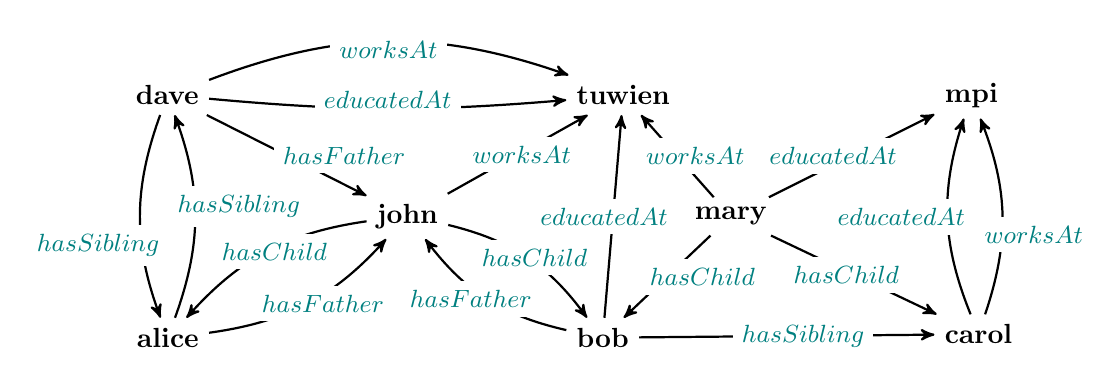
\begin{tikzpicture}[->,>=stealth',auto,node distance=3cm,
  thick,main node/.style={font=\bfseries}]

  \node[main node] (1) {john};
  \node[main node] (2) [right=3cm of 1] {mary};
  \node[main node] (3) [below left=1cm and 2cm of 1] {alice};
  \node[main node] (4) [below right=1cm and 1.5cm of 1] {bob};
  \node[main node] (5) [below right=1cm and 2cm of 2] {carol};
  \node[main node] (6) [above left=1cm and 2cm of 1] {dave};
  \node[main node] (7) [above right=1cm and 1.5cm of 1] {tuwien};
  \node[main node] (8) [above right=1cm and 2cm of 2] {mpi};

  \path[every node/.style={color=teal,fill=white,font=\small}]
    (1) edge node [right=-20pt] {$\mi{worksAt}$} (7)
    (2) edge node [right=-15pt] {$\mi{worksAt}$} (7)
    (4) edge node [right=-30pt] {$\mi{educatedAt}$} (7)
    (2) edge node [right=-10pt] {$\mi{hasChild}$} (4)
    (2) edge node [left=-20pt] {$\mi{hasChild}$} (5)
    (1) edge[bend left=20] node [right=-20pt] {$\mi{hasChild}$} (4)
    (4) edge[bend left=20] node [left=-20pt] {$\mi{hasFather}$} (1)
    (1) edge[bend right=20] node [right=-20pt] {$\mi{hasChild}$} (3)
    (3) edge[bend right=20] node [right=-20pt] {$\mi{hasFather}$} (1)
    (2) edge node [left=-20pt] {$\mi{educatedAt}$} (8)
    (5) edge[bend left=20] node [left=-10pt] {$\mi{educatedAt}$} (8)
    (5) edge[bend right=20] node [right=-10pt,pos=0.4] {$\mi{worksAt}$} (8)
    (6) edge node [right=-5pt] {$\mi{hasFather}$} (1)
    (3) edge[bend right=20] node [right=-10pt,pos=0.55] {$\mi{hasSibling}$} (6)
    (6) edge[bend right=20] node [left=-10pt,pos=0.65] {$\mi{hasSibling}$} (3)
    (6) edge[bend left=20] node [above=-10pt] {$\mi{worksAt}$} (7)
    (6) edge[bend right=5] node [below=-10pt] {$\mi{educatedAt}$} (7)
    (4) edge node [right=-20pt] {$\mi{hasSibling}$} (5)
    ;
\end{tikzpicture}
\caption{Example KG: family relations, working and education places.}
\label{fig:fam_grad}
\end{figure}
%\item 

\noindent \textbf{Completeness Confidence.} First, incompleteness information is used to determine whether to consider an instance in the unknown part of the rule as a counterexample or not. Formally, the \emph{completeness confidence} is defined as follows:
\begin{align*}
\mi{conf_{comp}}(r,\cG) := \frac{\textit{r-supp}(r,\cG)}{\textit{b-supp}(r,\cG) - \mi{npi}(r,\cG)}
\end{align*}
\begin{example}
Consider the KG $\cG'$ in Figure \ref{fig:fam_grad}
and the following cardinality statements for it:\\
$\mi{num(hC,john,\cG'^i)}\!=\!\mi{num(hC,mary,\cG'^i)}\!=3$; $\mi{num(hC,alice,\cG'^i)}\!=\!1$; \\
$\mi{num(hC,carol,\cG'^i)}\!=\!\mi{num(hC,dave,\cG'^i)}\!=\!0$;\\
$\mi{num(hS,alice,\cG'^i)}\!=\!\mi{num(hS,carol,\cG'^i)}\!=\!\mi{num(hS,dave,\cG'^i)}\!=\!2$;\\ 
$\mi{num(hS,bob,\cG'^i)}\!=\!3$;\\
where $hC$, $hS$ stand for $hasChild$ and $hasSibling$, correspondingly. We have:\\
$\mi{miss(hC,mary,\cG')}\!=\!\mi{miss(hC,john,\cG')}\!=\!\mi{miss(hC,alice,\cG')}\!=\!1$;\\ 
$\mi{miss(hC,carol,\cG')}\!=\!\mi{miss(hC,dave,\cG')}\!=\!0$;\\
$\mi{miss(hS,bob,\cG')}\!=\mi{miss(hS,carol,\cG')}\!=\!2$;\\
$\mi{miss(hS,alice,\cG')}\!=\!\mi{miss(hS,dave,\cG')}\!=\!1$;\\
%Also consider the following two extracted rules: 
For the rules $r_1'$ and $r_2'$ introduced above we have
% \vspace{-\topsep}
% \begin{align*}
% -\ r_3 &: hasChild(X,Y) \leftarrow worksAt(X,Z), educatedAt(Y,Z)\\
% -\ r_4 &: hasSibling(X,Z) \leftarrow hasFather(X,Y), hasChild(Y,Z)
% \end{align*}
 $\mi{conf_{comp}(r_1', \cG')}=\frac{2}{6}$ and $\mi{conf_{comp}(r_2', \cG')}=\frac{1}{2}$, which establishes the desired rule ranking.
\qed
\end{example}
%\item

\noindent \textbf{Completeness Precision and Recall.} In the spirit of information retrieval, the notions of \emph{completeness precision} and \emph{completeness recall} are defined to measure rule quality based on their predictions in complete and incomplete KG parts:
\begin{align*}
\mi{precision_{comp}}(r,\cG)=1-\frac{\mi{npc}(r,\cG)}{\textit{b-supp}(r,\cG)},\;\;\;
\mi{recall_{comp}}(r,\cG)=\frac{\mi{npi}(r,\cG)}{\sum_X \mathit{miss}(h,X,\cG)}
\end{align*}
Intuitively, rules having high precision are rules that predict few facts in complete parts, while rules having high recall are rules that predict many facts in incomplete ones. Rule scoring could also be based on any weighted combination of these two metrics.
%The \emph{recall measure} is similar to classical support measures, but now expresses how many facts on KG parts known to be incomplete, are generated by the rule (the more the better). The \emph{precision measure}, in turn, assesses how many of the generated facts are definitely wrong, namely those in complete parts (the more of these, the worse the rule). In fact, this is an upper bound on the precision, as the other facts cannot be evaluated.
\begin{example}
We have $\mi{npi(r_1', \cG')}\!=\!2$, $\mi{npc(r_1', \cG')}\!=\!4$, while $\mi{npi(r_2',\cG')}\!=\!4$, $\mi{npc(r_2,\cG')}\!=\!1$, resulting in $\mi{precision_{comp}(r_1,\cG')}\!=\!0.5$, $\mi{recall_{comp}(r_1',\cG')}\!\approx\!0.67$,and $\mi{precision_{comp}(r_2',\cG')}\!\approx\!0.83$, $\mi{recall_{comp}(r_2',\cG')}\!\approx\!0.67$.
\qed
\end{example}
%\item 

\noindent\textbf{Directional Metric.} If rule mining does make use of completeness information, and both do not exhibit any statistical bias, then intuitively the rule predictions and the (in)complete areas should be statistically independent. On the other hand, correlation between the two indicates that the rule-mining is \emph{(in)completeness-aware}. Hence, \emph{directional metric} is proposed following this intuition by measuring the proportion between predictions in complete and incomplete parts:
\begin{align*}
\mi{dm}(r,\cG) := \frac{\mi{npi}(r,\cG)-\mi{npc}(r,\cG)}{2\cdot(\mi{npi}(r,\cG)+\mi{npc}(r,\cG))}+0.5
\end{align*}
Since the real-world KGs are often highly incomplete, it might be reasonable to put more weight on predictions in complete parts. This can be done by multiplying predictions made in complete parts by a certain factor. This leads to the consideration of the weighted combination of a existing association rule measure $rm$, e.g., standard confidence or conviction, and 
the directional metric, using a weighting factor $\beta \in [0..1]$. Formally:
\begin{align*}
\mi{weighted\_dm}(r,\cG)=\beta \cdot \mi{rm}(r,\cG) + (1-\beta) \cdot \mi{dm}(r,\cG) 
\end{align*}
\begin{example}
We have $\mi{dm(r_1',\cG')}\approx 0.33$ and $\mi{dm(r_2',\cG')}=0.8$. With weighted directional metric using standard confidence ($rm = conf$), for $\beta=0.5$, we get $\mi{weighted\_dm(r_1',\cG')} \approx 0.29$ and $\mi{weighted\_dm(r_2',conf,\cG')} \approx 0.48$. \qed
\end{example}
%\end{itemize}

%\subsubsection{OP (Ontological Pathfinding).}
\subsubsection{Optimized Rule Evaluation}
% \thi{i think we should remove this section and just add citation}.\ds{shifted this part to rule evaluation}
% Learning rules from knowledge graph consists of two phases: constructing the rules and examining their quality based on the KG.
Most of state-of-the-art rule mining systems parallelize only the rule construction phase, while the quality of the rules are determined in a single thread. Huge size og KGs such as YAGO or Freebase %might 
%contain %hundreds million of entities and 
% billions of facts, thus  
%between them, Hence, 
prohibits their storage in %it is often impossible to store these KGs in 
a single machine. Therefore, % these rule mining systems either cannot scale to this size to
%the process of determine the rules' 
the rule quality estimation %, or they have to assign this task 
is usually delegated to some third-party database management system.
In practice this might not always be effective. % such as SQL, SPARQL \cite{amie}, which might not always be effective.

The focus of a recent % the novel 
 \emph{ontological pathfinding} (OP) \cite{op} algorithm is % not at how to find the candidate rules in the knowledge graph, but rather at
% how to 
the efficient examination of the rule's quality. % The rule construction step of OP algorithm relies on the relational pathfinding method . The only difference is that, instead of finding paths on the entity-relations graph, OP looks at the domain-range schema graph \cite{op}.
After candidate rules are constructed relying on a variation of \cite{DBLP:conf/aaai/RichardsM92}, their quality is determined via a sequences of parallelization and optimization methods including KG partitioning, joining and pruning strategies.

%\ds{Maybe we could insert other optimized evaluation methods here?} 



%%Recent works, e.g., \cite{cardinality-extraction-iswc-2016} focused on the task of extracting such cardinality information from text.We now discuss possible ways of making use of such information in rule scoring and ranking, which are core steps in association rule learning. A variety of measures for ranking rules have been proposed, with prominent ones being confidence, conviction and lift.  The existing (in-)completeness-aware rule measure in the KG context (the PCA confidence \cite{amie}) has two apparent shortcomings: First,  it only counts as counterexamples those %objects pairs $(x,y)$ for which at least one $h(x,y')$ %other facts 
%%with the head predicate $\mi{h}$ 
%%holds is in $\cG^a$ for some $\mi{y'}$ and a rule's head predicate $h$. This means it may incorrectly give high scores to rules predicting facts for very incomplete relations, e.g., \emph{place of baptism}. Second, it is not suited for data in non-functional relations that is not added in batches, such as awards, where the important ones are added instantly, while others much slower or even possibly never. 
%
%
%%Before dwelling into the details of our approach we discuss the formal representation of such meta-data. 
%
%%\leanparagraph{Cardinality Statements}
%%Overall, one can think of 6 different cardinality templates obtained by fixing subject, predicate or object in a triple and report the number of respective facts that hold in $\cG^i$. 
%%The lattice of possible basic (in)completeness templates on the fact level is presented in Fig.~\ref{fig:cs} 
%%on an example triple $\langle\mi{john\;hasChild\;mary}\rangle$. By fixing subject, predicate or object in a triple overall we obtain 6 different templates.
% %statements for these templates 
%% Ideally, we would be willing to possess and exploit numerical statements for all of these templates. For example,
%E.g., for $\mi{\tuple{john\;hasChild\;mary}}$ we %can construct the following cardinality assertions: 
%can count
%(1) children of $\mi{john}$ %has $\mi{n}$ children; 
%(2) edges from $\mi{john}$ to $\mi{mary}$; % there are $n$ edges; 
%(3) incoming edges to $\mi{mary}$; % has $n$ incoming $\mi{hasChild}$ edges; 
%(4) %there are $\mi{n}$ 
%facts with $\mi{john}$ as a subject; (5) %there are $n$ 
%facts over $\mi{hasChild}$ relation; (6) %there are $\mi{n}$ 
%facts with $\mi{mary}$ as an object. 
%
%In practice, numerical statements for templates (1) and (3) can be obtained using web extraction techniques \cite{cardinality-extraction-iswc-2016}, from functional properties of relations or from crowd-sourcing. For other templates things get trickier; one might be able to learn  
%them from the data or they could be defined by domain experts in topic-specific KGs. We leave this issue for future work, and focus here only on templates (1) and (3), which could be rewritten as the instances of the template (1) provided that inverse relations can be expressed in a KG. For instance, $\# s: \mi{hasChild}(s,\mi{john})=\# o: \mi{hasParent}(\mi{john},o)$ for the predicates $\mi{hasChild}$ and $\mi{hasParent}$, which are %in an 
%inverses of one another. % relation. 
%
%We represent the (in)completeness meta-data using cardinality statements by reporting (the numerical restriction on) the absolute number of facts over a certain relation in the ideal graph $\cG^i$. More specifically, we define the partial function $num$ that takes as input a predicate $\mi{p}$ and a constant $\mi{s}$ and outputs a natural number corresponding to the number of facts in $\cG^i$ over $\mi{p}$ with $\mi{s}$ as the first argument: 
%
%\begin{equation}\label{eq:num}
%\mi{num}(p,s) := \# o : p(s,o) \in \cG^i 
%\end{equation}
%
%Naturally, the number of missing facts for a given $p$ and $s$ can be obtained as
%
%\begin{equation}\label{eq:miss}
%\mi{miss}(p,s) := \mi{num(p,s)} - \#o : p(s,o) \in \cG^a %\setminus \cG^a
%\end{equation}
%
%\begin{example}
%\label{ex:cardinality}
%Consider the KG in Fig.~\ref{fig:fam_grad}.
%%and the rules $\mi{r1}$ and $\mi{r_2}$ from Example~\ref{ex:conf},
%%along with the following 
%%The following 
%and the following cardinality statements for it: %it might be available:
%\vspace{-\topsep}
%\begin{itemize}
%\setlength{\parskip}{0pt}
%\setlength{\itemsep}{0pt plus 1pt}
%\item $\mi{num(hasChild,john)}\!=\!\mi{num(hasChild,mary)}\!=3$; $\mi{num(hasChild,alice)}\!=\!1$;\\  $\mi{num(hasChild,carol)}\!=\!\mi{num(hasChild,dave)}\!=\!0$;
%\item $\mi{num(hasSibling,bob)}\!=\!3$;
%      $\mi{num(hasSibling,alice)}\!=\!\mi{num(hasSibling,carol)}\!=\!\mi{num(hasSibling,dave)}\!=\!2$.
%\end{itemize}
%\vspace{-\topsep}
%We then have:
%\vspace{-\topsep}
%\begin{itemize}
%\setlength{\parskip}{0pt}
%\setlength{\itemsep}{0pt plus 1pt}
%\item $\mi{miss(hasChild,mary)}\!=\!\mi{miss(hasChild,john)}\!=\!\mi{miss(hasChild,alice)}\!=\!1$;\\
%      $\mi{miss(hasChild,carol)}\!=\!\mi{miss(hasChild,dave)}\!=\!0$; 
%\item $\mi{miss(hasSibling,bob)}\!=\mi{miss(hasSibling,carol)}\!=\!2$;\\ 
%      $\mi{miss(hasSibling,alice)}\!=\!\mi{miss(hasSibling,dave)}\!=\!1$.\qed
%\end{itemize}
%\end{example}
%
%
%We are now ready to 
%define the \emph{completeness-aware rule scoring problem}.
%%\begin{problem}[Completeness-aware rule scoring] 
%Given a KG and a set of 
%%(in-)-complete\-ness
%cardinality statements, \emph{completeness-aware rule scoring} aims to score rules not only by their predictive power on the known KG, but also wrt.\ the number of wrongly predicted facts  
%in complete areas and the number of newly predicted 
%facts in known incomplete areas.
%%\end{problem}
%
%In the following we discuss and compare  
%three novel approaches for completeness-aware rule scoring. These are (i) the \emph{completeness confidence}, (ii) \emph{completeness precision} and \emph{recall}, 
%and (iii) \emph{directional metric}.
%Henceforth, all examples 
%consider the KG in Fig.~\ref{fig:fam_grad}, 
%rules from Ex.~\ref{ex:conf}, and cardinality statements  described in Ex.~\ref{ex:cardinality}.
%
%\leanparagraph{Completeness Confidence} In this work we propose to explicitly rely on incompleteness information in determining whether to consider an instance as a counterexample for a rule at hand or not.
%
%To do that, we first define two indicators for  a given rule $r: %\vec{H}
%\mi{h(X,Y)}\leftarrow \vec{B}$, %with $\vec{H}=h(X,Y)$, 
%reflecting the number of new 
%predictions made by $\mi{r}$ in incomplete ($\mi{npi(r)}$) and, respectively, complete ($\mi{npc(r)}$) KG parts:
%
%
%
%\begin{equation}
%\mi{npi}(r) := \sum_x min(\#y: h(x,y)\in \cG^a_r\backslash \cG^a, \mi{miss}(h,x))
%\end{equation}
%\vspace{-\topsep}
%\begin{equation}
%\mi{npc}(r) := \sum_x max(\#y: h(x,y)\in\cG^a_r\backslash \cG^a - \mi{miss}(h,x), 0)
%\end{equation}
%
%Note that summation is done exactly over those entities for which $\mi{miss}$ is defined.
%Exploiting these additional indicators 
%for %a given 
%$r:\,h(X,Y)\leftarrow \vec{B}$ we obtain the following \emph{completeness-aware confidence}:
%
%\begin{equation}\label{eq:comp_conf}
%\mi{conf_{comp}}(r) := \frac{\mi{supp}(r)}{\mi{supp}(\vec{B}) - \mi{npi}(r)}
%\end{equation}
%
%\begin{example}\label{ex:fam_grad}
%\label{ex:conf_comp}
%%Consider the KG in Fig.~\ref{fig:fam_grad}, rules $\mi{r1}$ and $\mi{r_2}$ from Example~\ref{ex:conf}, and cardinality statements mentioned in Example~\ref{ex:cardinality}.
%Obviously, the rule $\mi{r_2}$ %is
%should be preferred over $\mi{r_1}$. For our novel %This desired rule ranking is achieved by exploiting our novel 
%completeness confidence, we get %giving 
%$\mi{conf_{comp}(r_1)}=\frac{2}{6}$ %{5}$ 
%and $\mi{conf_{comp}(r_2)}=\frac{1}{2}$, resulting in the desired rule ordering,  which is not achieved by %is in contrast to 
%existing measures. %while the %previously introduced 
%The existing %ranking 
%metrics result in an incorrect rule ordering 
%%(see Ex.~\ref{ex:conf} and~\ref{ex:conf_pca}).
%\qed
%%%%%% OLD EXAMPLE %%%%%
%%\begin{example}\label{ex:fam_grad}
%%Consider the KG in Fig.~\ref{fig:fam_grad} along with the following cardinality statements:\\ $\mi{num(hasChild,mary)=num(hasChild,john)=3,num(hasChild,alice)=0}.$ 
%%Assume that the rules $\mi{r1}$ and $\mi{r_2}$ were mined from this KG.
%
%%\begin{itemize}
%%\item $\mi{r_1:\,hasChild(X,Y)\leftarrow worksAt(X,Z),graduateOf(Y,Z)}$
%%\item $\mi{r_2:\,hasChild(X,Y)\leftarrow hasParent(Y,X)}$;
%%\end{itemize}
%
%%Obviously, rule $\mi{r_1}$ is preferred over $\mi{r_2}$. This desired rule ranking in achieved by exploiting our novel completeness confidence, while the previously introduced ranking metrics result in an incorrect rule ordering.
%%\begin{itemize}
%%\item $\mi{conf(r_1)=2/3,conf(r_2)=2/5}$
%%\item $\mi{conf_{pca}(r_1)=1,conf_{pca}(r_2)=2/5}$
%%\item $\mi{conf_{comp}(r_1)=1/3,conf_{comp}(r_2)=1}$ \qed
%%\end{itemize}
%%%%%%%%%%%%%%%%%%%%%%%%
%
%
%\end{example}
%
%%The proposed metric generalizes %over 
%Our completeness confidence generalizes both 
%the standard %confidence 
%and the PCA confidence:
%
%\begin{proposition}
%For every KG $\cG$ and rule $r$ it holds that 
%\begin{itemize}
%\item[(i)] under the Closed World Assumption (CWA) $\mi{conf_{comp}(r)=conf(r)}$;
%\item[(ii)] under the Partial Completeness Assumption (PCA) $\mi{conf_{comp}(r)=conf_{pca}(r)}$.
%\end{itemize}
%\end{proposition}
%
%\begin{proof}
%\textbf{(i)} Under the CWA, it holds that for all $ p\in \mathbf{R},\,s\in \cC: \mi{miss}(p,s) = 0$. Thus, for all rules $r$, we have that $\mi{npi}(r) = 0$, and hence, $\mi{conf_{comp}(r)}=\mi{conf(r)}$.
%\smallskip
%
%\noindent \textbf{(ii)} Under the PCA, it is assumed that for all $p\in \mathbf{R}$ and $s \in \cC$ it holds that 
%$\mi{miss}(p,s) = 0$ if $\exists o: p(s,o)\in \cG^a$. We extend the PCA by assuming that $miss(p,s)=+\infty$ for KG parts for which cardinality statements are unavailable, which is a reasonable assumption given the overall incompleteness of the available KG, i.e., 
%%and otherwise, 
%$\mi{miss}(p,s) = +\infty$. 
%%, since the number of missing facts is unrestricted. 
%Hence, for all $r$ we have
%$\mi{npi(r)=\sum_{x}predict(r,x)}$, where
%
%\begin{center}
%$predict(r,x)=
%\begin{cases}
%0, \text{ if } \exists y: h(x,y)\in \cG^a\\
%\#y: h(x,y) \in \cG^a_r\backslash \cG^a, \text{ if } \forall y': h(x,y')\not\in \cG^a\\
%\end{cases}$
%\end{center}
%From this we get
%
%\begin{center}
%$\mi{conf_{comp}(r)=\dfrac{supp(r)}{supp(\vec{B})-\sum_{x: \forall y': h(x,y')\not\in\cG^a}\#y: h(x,y)\in \cG^a_r\backslash \cG^a}}$
%\end{center}
%
%The denominator of the latter formula counts all rule body and subtracts from them those, for which the head $h(x,y)$ is predicted and $\forall y':h(x,y')\not \in \cG^a$. Hence, we end up counting only  body substitutions with $h(x,y')\in \cG^a$ for at least  one $y'$, i.e., $\mi{\#(x,y):\exists \vec{Z}:\vec{B}\wedge \exists y': h(x,y')\in \cG^a}$, from which the result follows. \qed
%
%\end{proof}
%
%
%
%In other words, if %we assume that 
%the graph is known to be fully complete, i.e., for all $p \in\cR,s\in\cC$ we have
%$\mi{miss}(p,s)=0$ , then $\mi{conf_{comp}}$ is the same as the standard confidence. Similarly, if  $\mi{miss}(p,s)= 0$ for such $p,s$ pairs that at least one 
%fact $p(s,\_)\in \cG^a$ exists and  $\mi{miss}(p,s) = +\infty$ for the rest,  
%then $\mi{conf_{comp}}$ is the same as the PCA confidence.
%
%\leanparagraph{Completeness Precision and Recall} Further developing the idea of scoring rules based on their predictions in complete and incomplete KG parts, we propose to consider the notions of  \emph{completeness precision} and \emph{recall}\footnote{For brevity we skip the word "completeness" if clear from the context.} for rules defined in the spirit of information retrieval. Intuitively, rules having high precision are rules that predict few facts in complete parts, while rules having high recall are rules that predict many facts in incomplete ones. Rule scoring could then be based on any weighted combination of these two metrics.
%
%Formally, we define the precision and recall of a rule $\mi{r: h(X,Y)\leftarrow \vec{B}}$ as follows:
%
%\begin{equation}\label{eq:precision}
%\mi{precision_{comp}}(r)=1-\frac{\mi{npc}(r)}{\mi{supp}(\vec{B})}
%\end{equation}
%
%\begin{equation}\label{eq:recall}
%\mi{recall_{comp}}(r)=\frac{\mi{npi}(r)}{\sum_s \mathit{miss}(h,s)}
%\end{equation}
%
%The \emph{recall measure} is similar to classical support measures, but now expresses how many facts on KG parts known to be incomplete, are generated by the rule (the more the better). The \emph{precision measure}, in turn, assesses how many of the generated facts are definitely wrong, namely those in complete parts (the more of these, the worse the rule). In fact, this is an upper bound on the precision, as the other facts cannot be evaluated.
%
%\begin{example}
%\label{ex:prec_recall}
%%Consider the KG in Fig.~\ref{fig:fam_grad}, rules $\mi{r1}$ and $\mi{r_2}$ from Example~\ref{ex:conf}, and cardinality statements from Example~\ref{ex:cardinality}. 
%It holds that $\mi{npi(r_1)}\!=\!2$, %1$, 
%$\mi{npc(r_1)}\!=\!4$, %3$, 
%while $\mi{npi(r_2)}\!=\!4$, $\mi{npc(r_2)}\!=\!1$, resulting in $\mi{precision_{comp}(r_1)}\!=\!0.5$, 
%$\mi{recall_{comp}(r_1)}\!\approx\!0.67$, %0.5$, 
%and $\mi{precision_{comp}(r_2)}\!\approx\!0.83$, $\mi{recall_{comp}(r_2)}\!\approx\!0.67$, which lead to the expected relative rule ordering. \qed
%\end{example}
%%%%%% OLD EXAMPLE %%%%%
%%\begin{example}
%%Consider the KG in Fig.~\ref{fig:fam_grad} and the rules $\mi{r_1}$ and $\mi{r_2}$ from Example~\ref{ex:conf}. It holds that $\mi{npi(r_2)=3}$, $\mi{npc(r_2)=0}$, while $\mi{npi(r_1)=0}$ and $\mi{npc(r_1)=1}$. From this we obtain $\mi{precision(r_2)=recall(r_2)=1}$, and $\mi{precision(r_1)=0}$, $\mi{recall(r_1)=0}$, leading to the expected relative rule ordering. \qed
%%\end{example}
%%%%%%%%%%%%%%%%%%%%%%%%
%
%\leanparagraph{Limitations}
%While precision and recall are insightful when there are sufficiently many predictions made in (in-)complete %/incomplete 
%parts, they fail when the number of (in-)completeness statements in comparison with the KG size is small. Consider, for instance, a rule that predicts 1000 new facts over $\mi{hasChild}$ relation, out of which 2 are in complete, and 2 are in incomplete parts, and 
%overall 
%1 million children are missing. 
%%in total. 
%This would imply a precision of 99.8\%, and a recall of 0.0002\%, both of which are 
%not very informative.
%
%Therefore, next we propose to look at the difference between  
%expected numbers of predictions in complete and incomplete parts, or simply at their ratio.
%
%\leanparagraph{Directional Bias} If rule mining does make use of completeness information, and both do not exhibit any statistical bias, then intuitively the rule predictions and the (in)complete areas should be statistically independent. On the other hand, correlation between the two indicates that the rule-mining is \emph{(in)completeness-aware}. 
%
%\begin{example}
%Suppose in total a given KG stores 1 million humans, and we know that 10,000 (1\%) of these are missing some children (incompleteness information), while we also know that 1000 of the persons are definitely complete for children (0.1\%). Let the set of rules mined from a KG predict 50,000 new facts for the $\mi{hasChild}$ relation. Assuming independence between predictions and (in)completeness statements, we would expect 1\% out of 50,000, i.e., 500 facts to be predicted in the incomplete areas and 0.1\%, i.e., 50 in the complete KG parts. If instead we find 1000 children predicted for people that are missing correspondingly many children, and 10 for people that are not missing these, the former deviates from the expected value by a factor of 2, and the latter by a factor of 5.
%\end{example}
%%
%%
%Following the intuition from the above example, we propose to look at the extent of the non-independence to quantify the (in)completeness-awareness of rule mining. Let us consider predictions made by rules in a given KG, where \textit{E(\#facts)} is the expected number of predictions and $\alpha=0..1$ is the weight given to completeness versus incompleteness. Then the directional coefficient of a rule $r$ is defined as follows:
%
%\begin{equation}\label{eq:direct_coef}
%\mi{direct\_coef}(r) := \alpha \cdot \frac{E(\mi{npc}(r))}{\mi{npc}(r)} + (1-\alpha) \cdot \frac{\mi{npi}(r)}{E(\mi{npi}(r))}
%\end{equation}
%Unlike the other measures that range from 0 to 1, the directional coefficient takes values between 0 and infinity, where 1 is the default. If the ratio between the KG size and the size of the (in)complete parts is the same as the ratio between the %size of 
%predictions in the (in)complete parts and their total number, i.e.,
%%number of predictions, i.e., 
%if the directional coefficient is 1, then the statements do not influence the rule at all.
%The higher is the \emph{directional coefficient}, the more ``\emph{completeness-aware}'' the rules are.
%
%In practice, expected values might be difficult to compute, and statistical independence is a strong assumption. An alternative that does not require knowledge about expected values is to directly measure the proportion between predictions in complete and incomplete parts. We call this the \emph{directional metric}, which is computed as
%%
%\begin{equation}\label{eq:direct_metric}
%\mi{direct\_metric}(r) := \frac{\mi{npi}(r)-\mi{npc}(r)}{2\cdot(\mi{npi}(r)+\mi{npc}(r))}+0.5\\
%\end{equation}
%%
% The metric is based on the same ideas as the directional coefficient, but does not require knowledge about the expected number of predictions in complete/incomplete KG parts. It is designed to range between 0 and 1 again, thus allowing convenient weighting with other $[0, 1]$  measures.
%The directional metric of a rule that predicts the same number of facts in incomplete as in complete parts is %, has a value of 
%0.5, a rule that predicts twice as many facts in incomplete parts has a value of 0.66, and so on.
%
%Since the real-world KGs are often highly incomplete, it might be reasonable to put more weight on predictions in complete parts.
%This can be done by multiplying predictions made in complete parts by a certain factor. We propose to consider the combination of a weighted existing association rule measure, 
%e.g., confidence or conviction and 
%the directional metric, %i.e.,
%with the weighting factor  %is 
%$\beta=0..1$. Using confidence, we obtain  
%\begin{equation}\label{eq:direct_metric_score}
%\mi{weighted\_dm}(r)=\beta \cdot \mi{conf}(r) + (1-\beta) \cdot \mi{direct\_metric}(r) 
%\end{equation}
%
%
%\begin{example}
%We get $\mi{direct\_metric(r_1)}{\approx} 0.33$ and $\mi{direct\_metric(r_2)}{=}0.8$. %Furthermore, %assuming 
%For $\beta=0.5$ and %standard 
%confidence %from Ex.~\ref{ex:conf}, %we get 
%$\mi{weighted\_dm(r_1)} \approx 0.29$ and $\mi{weighted\_dm(r_2)} \approx 0.48$. \qed
%\end{example}
%
%\leanparagraph{Acquisition of Numerical Statements}
%\label{sec:acquisition-numerical}
%As we have shown, exploitation of numerical (in-)completeness statements is very beneficial for rule quality assessment. 
%A natural question is where to acquire such statements from in real-world settings.  
%Various works have shown that numerical 
%assertions can be 
%frequently found on the Web~\cite{rdfcomp}, %can be 
%obtained via crowd-sourcing~\cite{DarariREN16}, text mining~\cite{paramita-acl-2017} or completeness rule mining~\cite{galarragapredicting}. 
%We believe that mining %rules about 
%numerical correlations concerning KG edges and then 
%assembling %these 
%them into rules %to rules about completeness, 
%is a valuable and a %more 
%modular approach to obtain further completeness information, which we sketch in what follows. 
%
%We start with an available KG $\cG^a$ and some statements of the form (\ref{eq:num}).
%
%
%%\leanparagraph{Approach}
%%We now sketch an approach for mining rules that can be applied to predict numerical restrictions on facts of a certain form using the available cardinality statements and the data in the KG as input. 
%
%\leanparagraph{Step 1} For every cardinality  $\mi{num(p,s)}=k$, we create the facts $p_{\leq k}(s)$ and $p_{\geq k}(s)$. For the pairs $p\in\mathbf{R},s\in\cC$  with no available cardinality statements we construct the facts $p_{\geq \# o: p(s,o)\in \cG^a}(s)$,  encoding that outgoing $p$-edges from $s$ might be %some facts over $p$ with $s$ being the first argument might be 
%missing in $\cG^a$, as the graph is believed to be incomplete by default.
%Here, $p_{card}$ with $\mi{card\in \{\leq \_, \geq \_\}}$ are fresh unary predicates not present in $\Sigma_{\cG^a}$, which describe (bounds on) the number of outgoing $p$-edges for a given constant. We store all constructed facts over $p_{\mi{card}}$ in %a temporary set 
%$\cS$.
% 
%We then complete the domain of each $p_{\mi{card}}$ predicate as follows. For every $p_{\leq k}(s)\in \cS$, if $p_{\leq k'}(s')\in\cS$ for some $s'\in \cC$ and $k' > k$, we construct the rule $ p_{\leq k'}(X)\leftarrow p_{\leq k}(X).$ Similarly, for every $p_{\geq k}(s)\in\cS$, if $p_{\geq k'}(s')\in \cS$ where $k' < k$, we create $p_{\geq k'}(X)\leftarrow p_{\geq k}(X)$.
%%introduced unary predicate 
%The constructed rules are then applied to the facts in $\cS$ to obtain an extended set $\cG^{\mi{card}}$ of facts over $p_{\mi{card}}$. The latter step is crucial when using a rule mining system that is not doing arithmetic inferences (like $x>4$ implies $x>3$).
%%by exhaustively applying the two rules %$p_{\geq k}(s) \leftarrow p_{\geq k+1}(s)$
%%$p_{\geq k}(X) \leftarrow p_{\geq k'}(X)$ where $k < k'$
%%and $p_{\leq k}(X)\leftarrow p_{\leq k'}(X)$ where $k > k'$.
%%$p_{\leq k+1}(s) \leftarrow p_{\leq k}(s)$ 
%%until saturation.
%%This process materialize fully all "interesting" predicated: it is only interesting to consider $p_{\leq 0}$ and the predicates $p_{\leq k+1}$ such that $\{ x \mid p_{\leq k+1}(x) \} \neq \{ x \mid p_{\leq k}(x) \}$ because, if not, then $\{ x \mid p_{\leq k+1}(x) \} = \{ x \mid p_{\leq k}(x) \}$ and, so, does not brings any new information (as we obviously have $\{ x \mid p_{\leq k+1}(x) \} \subseteq \{ x \mid p_{\leq k}(x) \}$). The same idea holds for $(p_{\geq k})_{k \in \mathbb{N}}$.\tptcomment{Previous sentences updated}
%%We denote the set of all such additional facts as $\cG^{\mi{card}}$.
%
%\leanparagraph{Step 2} We then use such a standard rule learning system, AMIE \cite{amie}, on $\cG^a \cup \cG^{\mi{card}}$ to mine rules like:
% 
%\vspace{-\topsep}
%\small{
% \begin{itemize}
%%\begin{minipage}{0.3\linewidth}
%\item[(1)] $\mi{p_{card}(X)\leftarrow p'_{card}(X)}$
%\item[(2)] $\mi{p_{card}(X)\leftarrow p'_{card}(X), p''_{card}(X)}$
%\item[(3)] $\mi{p_{card}(X)\leftarrow p'_{card}(X), r(X,Y)}$
%%\end{minipage}
%%\begin{minipage}{0.7\linewidth}
%\item[(4)] $\mi{p_{card}(X)\leftarrow p'_{card}(X), r(X,Y)},\mi{p''_{card}(Y)}$
%\item[(5)] $\mi{p_{card}(X)\leftarrow r(X,Y), p''_{card}(Y)}$
%%\end{minipage}
%\end{itemize}
%}\normalsize
%\vspace{-\topsep}
%\noindent We rank the obtained %se 
%rules based on confidence %based on standard %association 
%%rule measures 
%and select the top %$n$ rules 
%ones into the set $\cR$.
%
%\leanparagraph{Step 3} Finally, in the last step we use the obtained ruleset $\cR$ to derive further numerical statements together with weights assigned to them. For that we compute $\cG'=\bigcup_{r\in \cR}\{\cG^{card}\cup\cG^{a}\}_{r}$. The weights of the statements are inherited from the rules that derived them. We then employ two simple heuristics: (i) Given multiple rules predicting the same fact, the highest weight for it is kept. We then post-process predictions made by different rules for the same subject-predicate pair as follows. 
%(ii) If $p_{\leq k}(s),p_{\geq k'}(s)\in \cG'$ for $k'>k$, we remove from $\cG'$ predictions with the lowest weight thus resolving the conflict on the numerical bounds. %, and thus end up with a graph, in which none of the bounds on the number of edges represented by the dedicated facts contradict each other. 
%
%From the obtained graph we reconstruct cardinality statements as follows.
%\vspace{-\topsep}
%\begin{itemize}
%\item Given $p_{\leq k}(s),\mi{p_{\geq k}(s)}\in \cG'$ with weights $w$ and $w'$ %assigned to them, 
%we create a cardinality statement $\mi{num(p,s)=k}$ with the weight $min(w,w')$. % and add it to the set $\cS$. 
%\item If $p_{\leq k}(s),p_{\geq k'}(s) \in \cG'$ for $k'<k$, then we set $k' \leq \mi{num(p,s)} \leq k$.
%\item Among two facts $p_{\leq k}(s), p_{\leq k'}(s)$ (resp. $p_{\geq k}(s)$, $p_{\geq k'}(s)$) with $k<k'$ (resp. $k>k'$) the first ones are kept and represented similar to \ref{eq:num}. 
%\end{itemize}
%
%Regular facts in $\cG'$ are similarly translated into their numerical representations.
%%Note that we could end up with an infinite number of $p_{\leq k}$ unary predicates. But it is only interesting to consider $p_0$ and the predicates $p_{\leq k+1}$ such that $\{ x \mid p_{\leq k+1}(x) \} \neq \{ x \mid p_{\leq k}(x) \}$ because, if not, then $\{ x \mid p_{\leq k+1}(x) \} = \{ x \mid p_{\leq k}(x) \}$ and, so, does not brings any new information (as we obviously have $\{ x \mid p_{\leq k+1}(x) \} \subseteq \{ x \mid p_{\leq k}(x) \}$). The same idea holds for $(p_{\geq k})_{k \in \mathbb{N}}$.
%
%
%%%%%% Old KG %%%%%
%\iffalse
%\scriptsize
%\begin{table}[t]
%\begin{center}
%\renewcommand*{\arraystretch}{0.95}
%\begin{tabular}{|l|l|l|l|}
%\hline
%&  $\mi{hasBrother_{\geq 1}}$ &$\mi{hasSister_{\geq 1}}$&
%$\mi{hasSibling_{\geq 2}}$\\\hline
%$\mi{ann}$ & $\checkmark$ &$\checkmark$ &$\checkmark$\\ \hline
%$\mi{kate}$ & $\checkmark$ &$\checkmark$ &$\checkmark$\\ \hline
%$\mi{lola}$ & $\checkmark$ &$\checkmark$ &$\checkmark$\\ \hline
%$\mi{john}$ & $\checkmark$ &$\checkmark$ &\\ \hline
%\end{tabular}
%\caption{Meta-data from Example~\ref{ex:card}}
%\label{tab:inc}
%\end{center}
%\end{table}
%\normalsize
%\fi
%%%%%%%%%%%%%%%%%%%%
%
%%%%%% Old KG %%%%%
%\iffalse
%\begin{figure}[t]
%\begin{center}
%\includegraphics[width=.44\textwidth]{figures/fam}
%\caption{Example KG: family}
%\label{fig:fam}
%\end{center}
%\end{figure}
%\fi
%%%%%%%%%%%%%%%%%%%%
%
%%\simoncomment{This example may raise questions whether our language is good, as it would be better to learn parameterized rules such as c.parent.children=n $\rightarrow$ c.siblings=n-1, instead of c.parent.children=3 $\rightarrow$ c.siblings=2. Can we find another one?}
%
%\begin{example}
%Consider the KG in Fig.~\ref{fig:fam_grad}
%%and the rules $\mi{r1}$ and $\mi{r_2}$ from Example~\ref{ex:conf},
%%along with the following 
%%The following 
%and the following cardinality statements for it: $\mi{num(hasChild,john)\!=\!num(hasSibling,bob)}\!=\!3$.  %construct
%%We generate, between, others, 
%Among others, $\cG^{\mi{card}}$ contains the facts:
%%We generate the following graph with numerical facts 
%%for $\mi{hasChild}$ and $\mi{hasSibling}$ relations and obtain % extended version of the graph: 
%$%\cG^{\mi{card}}=\{
%\mi{hasChild_{\geq 3}(john)},
%\mi{hasSibling_{\geq 3}(bob)},
%\mi{hasChild_{\geq 2}(mary)},
%\mi{hasChild_{\geq 2}(john)},\\ 
%\mi{hasSibling_{\geq 2}(bob)},
%\mi{hasSibling_{\geq 1}(dave)}$, and
%$\mi{hasSibling_{\geq 1}(alice)}$. %,\cdots\}$.
%%On %this 
%On the graph $\cG^a\cup \cG^{\mi{card}}$, the confidence of $\mi{hasSibling}_{\geq 2}(X)\,{\leftarrow}\, \mi{hasFather}(X, Y), \mi{hasChild}_{\geq 3}(Y)$ %has a confidence of 
%is $\frac{1}{3}$ and
%1 for
%$\mi{hasSibling_{\geq 1}(X)\,{\leftarrow}\, hasFather(X, Y),hasChild_{\geq 3}(Y)}$. %has  %a 
%%confidence of $1$.
%\qed
%\end{example}
%
%%  From $\mi{hasParent(john, alice)}, hasChild_{\leq 3}$ and the rule $\mi{r_1}$ we obtain\\ $\mi{hasSibling_{\leq 2}(john)}$ with confidence 2/3, while from the facts in Tab.~\ref{tab:inc} and $\mi{r_2}$ we get $\mi{hasSibling_{\geq 2}(john)}$ with confidence 3/4. Since the facts that we have derived do not contradict each other, we can assume that the exact number of siblings for $\mi{john}$ is 2 with the confidence $min(2/3, 3/4) = 2/3$.
% 
% 
%%  The completeness knowledge from above would be encoded as $\mi{hasChild_{\leq 3}(tom)}$,\linebreak $\mi{hasChild_{\leq 3}(mary),  hasChild_{\leq 3}(alice)}$, $\mi{hasChild_{\geq 3}(tom), hasChild_{\geq 3}(mary)}$, $\mi{hasChild_{\geq 3}(alice)}$ and $\mi{hasSibling_{\geq 2}(pete)}$, $\mi{hasSibling_{\geq 2}(bob)}$. From this data we mine a rule of the form~(5):
%% \begin{center}
%% $\mi{r_1:\, hasSibling_{\leq 2}(X)\leftarrow hasParent(X,Y), hasChild_{\leq 3}(Y)}$
%% \end{center}
%%  stating that normally the number of persons siblings is at most 2 given that his parents have at most 3 children.
%%\end{example}
%
% Ideally, provided that sufficiently many similar numerical correlations about %for different 
% edge numbers %values 
%are extracted, one can induce more general hypothesis involving arithmetic functions like the number of person's siblings is bounded by the number of his parents' children plus 1 or the sum of person's brothers and sisters equals the number of his siblings.  %However, that will require complex induction using mathematical functions, which 
% We leave these more complex generalizations for future work. Similarly, the employed heuristic provide potential for more advanced voting/weighting schemes and inconsistency resolution in the case of conflicting cardinality assertions.
%

\section{Nonmonotonic Rule Learning}\label{sec:nmrulelearn}
So far we have considered approaches for constructing Horn rules. However,  these are not sufficiently expressive for representing incomplete human knowledge, and they are inadequate for capturing
exceptions. Thus, Horn rules extracted from the existing KGs can potentially %they %herefore, they 
predict erroneous facts as shown in Section~\ref{sec:intro}. 

In this section, we provide an overview of approaches for learning nonmonotonic rules from large and incomplete KGs. First, we describe a method that relies on cross-talk among the extracted rules to guess their exceptions~\cite{gad2016,rumis}. Then we present an approach that exploits embedding-based methods for knowledge graph completion during rule construction~\cite{thinh2018}.

\subsection{Revision-based Method}
Exception handling has been traditionally faced in ILP by learning non-monotonic logic programs \cite{DBLP:conf/ijcai/InoueK97,DBLP:journals/tocl/Sakama05,XHAIL,CorapiRL10,ILASP_system} (see Section~\ref{sec:reasoning}). However, most of the existing methods assume that the data from which the rules are induced is complete.

In \cite{gad2016} a revision-based approach for extracting exception-enriched (i.e., nonmonotonic) rules from incomplete KGs has been proposed. 
It pre-processes a KG by %translating
projecting all binary facts into unary ones applying a form of propositionalization technique \cite{propos} (e.g., $\mi{livesIn(brad,berlin)}$ could be translated to $\mi{livesInBerlin(brad)}$ or $\mi{livesInCapital(brad)}$ with obvious loss of information) and adapts data mining methods designed for transaction data to extract Horn rules, which are then augmented with negated atoms. In \cite{rumis} the approach has been extended to KGs in their original relational form. We now briefly summarize the ideas of  \cite{gad2016,rumis}.
% In \cite{ilp2016} the results from \cite{DBLP:conf/semweb/Gad-ElrabSUW16} to KGs in their original relational form.

In these works, the KG completion problem from Definition~\ref{def:kgcomp} is treated 
as a \emph{theory revision} task, where, given a KG and a set of (previously learned) Horn rules, the goal is to revise this set by adding exceptions, such that the obtained rules have higher predictive accuracy than the original ones. 

Since normally, the ideal graph $\cG^i$ is not available, in order to estimate the quality of a
revised ruleset, two generic quality functions $q_{\mi{rm}}$ and
$q_{\mi{conflict}}$ are devised, which both take as input a ruleset $R$ and a KG $\cG$ and output a
real value, reflecting the suitability of $R$ for data prediction.  More
specifically, 
\begin{equation}q_{\mi{rm}} (R,\cG)=\dfrac{\sum_{r\in
    R}rm(r,\cG)}{|R|}, \end{equation}
     where $\mi{rm}$ is some standard
association rule measure \cite{Azevedo2007}. %\gad{text updated here!} 
Conversely, $q_{\mi{conflict}}$ estimates the number of conflicting predictions that the rules in $R$ generate. To measure $\mi{q_{conflict}}$ for $R$,
 an extended set of rules $R^{aux}$ is created, %to materialize predictions prevented by the negative part of each individual rule in $R$. %, which
%$R^{aux}$ 
which contains every %every
revised rule in $R$ %and
together with %their
its auxiliary version. For a rule $r:\,h(X,Y)\leftarrow B,\naf\,E$ in $R$,
its auxiliary version $r^{\mi{aux}}$ is constructed by: i) transforming $r$ into a Horn rule by
removing %the negation
$\naf$ from negated body atoms, %in the exception body atom,
and ii) replacing the head
predicate $\mi{h}$ of $r$ %(e.g. $a$)
with a newly introduced predicate $\mi{not\_h}$ which intuitively should contain %will contain
%all
instances which are \emph{not} in $\mi{h}$. 

\begin{example} The auxiliary rule $r_2^{aux}$ for the rule $r_2$ from Section~\ref{sec:intro} is as follows $\mi{r_2^{aux}:\,not\_livesIn(Y,Z)\leftarrow marriedTo(X,Y),livesIn(X,Z),researcher(Y)}$, and it informally reflects that married people among whom one is a researcher often do not live together. For $\mi{r_3:\,livesIn(X,Y)\leftarrow bornIn(X,Y),\naf\ immigrant(X)}$ we similarly have $\mi{r_3^{aux}:\,not\_livesIn(X,Y)\leftarrow bornIn(X,Y),immigrant(X)}$. If $R=\{r_1,r_2\}$ then $R^{aux}=\{r_1,r_1^{aux},r_2,r_2^{aux}\}$. 

Intuitively, $q_{\mi{conflict}}(R,\cG)$ estimates the portion of conflicting predictions \\$\mi{livesIn(a,b),not\_livesIn(a,b)}$ made by the rules in $R^{aux}$. The hypothesis of \cite{gad2016,rumis} is that for a set $R$ of good rules with reasonable exceptions, the number of conflicting predictions produced by $R^{aux}$ is small.  \qed
\end{example}


%the original head predicate (e.g. $not\_a$).
Formally, based on statistics of both rules $r$ and $\mi{r^{aux}}$ in a set of exception-enriched rules $R$, the measure $\mi{q_{conflict}}$ is defined:

\begin{equation}
\mi{q_{conflict}(R,\cG)=\sum_{p\in pred(R)} \dfrac{|\vec{c}\,|\,p(\vec{c}),not\_p(\vec{c})\in \cG_{R^{\mi{aux}}}|}{|\vec{c}\,|\,not\_p(\vec{c})\in \cG_{R^{\mi{aux}}}|}}
\end{equation}
where $\mi{pred(R)}$ stores predicates appearing in $R$.
%\noindent where $\mi{pred(\cR^{\mi{aux}})}$ is the set of predicates appearing in $\cR^{\mi{aux}}$.$q_{\mi{conflict}}=$% Given a potentially incomplete graph $\cG^a$ and a set of Horn rules $\cR_H$
% mined from $\cG^a$, our goal is to add default negated atoms (exceptions) to the
% rules in $\cR_{H}$ and obtain a revised ruleset $\cR_{\mi{NM}}$ such that the
% set difference between $\cG^a_{\cR_{\mi{NM}}}$ and $\cG^i$ is smaller than
% between $\cG^a_{\cR_H}$ and $\cG^i$. If in addition the set difference between $\cG^a_{\cR_{\mi{NM}}}$ and $\cG^i$ is
% the smallest among the ones produced by other revisions $\cR_{\mi{NM}}'$ of
% $\cR_H$ then we call $\cR_{\mi{NM}}$ an \emph{ideal nonmonotonic} revision. For single
% rules such revision is defined as follows:
% \begin{definition}[Ideal nonmonotonic revision]\label{def:nmrev} Let
%     $G=(\cG^a,\cG^i)$ be an incomplete data source. Moreover, let
%     $r:\;a\leftarrow b_1,\dotsc, b_k$ be a Horn rule % in $\cR_{\mi{H}}$ (i.e.
%     mined from $\cG^a$. An \emph{ideal nonmonotonic revision} of $r$ \wrt\ $\cG$
%     is any rule \begin{equation}\label{eq:lp} r':\;\;a \leftarrow b_1,\dotsc,
%         b_k,\naf\ b_{k+1}, \naf\ b_n, \end{equation} such that $\cG^i \triangle
%     \cG^a_{r'}\subset \cG^i\triangle \cG^a_{r}$ \footnote{$\cG_1 \triangle
%     \cG_2=(\cG_1 \backslash \cG_2)\cup (\cG_2 \backslash \cG_1)$}, i.e. the
%     completion of $\cG^a$ based on $r'$ is closer to $\cG^i$ then the completion
%     of $\cG^a$ based on $r$, and $\cG^a_{r''}\triangle \cG^i\subset
%     \cG^a_{r'}\triangle \cG^i$ for no other nonmonotonic revision $r''\neq r'$
%     of $r$. If k=n, then the revision coincides with the original rule.  \end{definition}
% In our work, we assume that the ideal graph $\cG^i$ is not available (otherwise
% nothing would need to be learnt). Therefore, we cannot verify whether a revision
% is ideal for $\cR_{H}$. What we can do, however, is to estimate using some
% quality functions whether a given
% revision produces an approximation of $\cG^i$ that is better then the approximation produced by the original Horn
% ruleset. For this purpose, we introduce a generic quality function $q$ which
%  receives as input a revision $\cR_{\mi{NM}}$ of the ruleset $\cR_H$
%  and a graph $\cG$, and
%  returns a real value that reflects the quality of the revised set
%  $\cR_{\mi{NM}}$.

Formally, the problem targeted in \cite{gad2016,rumis} is formulated as follows: 
\begin{definition}[Quality-based Horn Theory Revision] Given a KG $\cG$,
a set of nonground Horn rules $R_{\mi{H}}$ mined from $\cG$, and a quality
function $\mi{rm}$, %$q$
find a set of rules $R_{\mi{NM}}$ obtained by
adding negated atoms to $\mi{body(r)}$ for some $r{\in} R_{H}$ s.t. (i)
${q_{\mi{rm}}(R_{\mi{NM}},\cG)}$ is maximal, and (ii)
${q_{\mi{conflict}}(R_{\mi{NM}},\cG)}$ is minimal.
\end{definition}

%More formally:\\ \\\noindent
%\textbf{Problem:} quality-based Horn rule revision

%\noindent \textbf{Given:} KG $\cG$, set of nonground Horn rules $\cR_{\mi{H}}$ mined from $\cG$,
% quality function $q$

%\noindent \textbf{Find:} set of rules $\cR_{\mi{NM}}$ obtained by adding negated atoms
%to $\mi{Body(r)}$ for some $r{\in} \cR_{H}$,\\\phantom{\textbf{Find:} } s.t. (i) $q_{\mi{rm}}(\cR_{\mi{NM}},\cG)$ is maximal, and
%(ii) $q_{\mi{conflict}}(\cR_{\mi{NM}},\cG)$ is minimal.
%\\ \\
%\noindent
Given huge size of KGs, finding the best possible revision is unfeasible in practice. Thus, in \cite{gad2016,rumis} a heuristics-based method that combines standard relational association rule mining techniques with a FOIL-like supervised learning algorithm \cite{foil} for computing exceptions has been proposed to find an approximate solution to the above problem (see Figure~\ref{fig:iswc_process} for overview). 

\begin{figure}[t]
\centering
\includegraphics[width=1\textwidth]{figures/overview_new}
\caption{Rule revision method for nonmonotonic rule learning~\cite{gad2016,rumis}.}
\label{fig:iswc_process}
\end{figure}
\noindent \textbf{Step 1.} After mining Horn rules using an off-the-shelf algorithm (e.g.,
 \cite{amie}), %can also be applied)
 one computes for each rule the \emph{normal} and
\emph{abnormal substitutions}, defined as

\begin{definition}[$r$-(Ab)Normal Substitutions]\label{sec:rulelearn}
Let $\cG$ be a KG, $\mi{r}$ a Horn rule mined from $\cG$, and let $\cV$ be a set of variables occurring in $r$. Then
\begin{myitemize}
\item $\mi{NS(r, \cG)=\{\theta\, |\, head(r)\theta,body(r)\theta \subseteq \cG\}}$ is an $\mi{r}$-normal set of substitutions;
\item $\mi{ABS(r, \cG){=}\{\theta'\, |\, body(r)\theta' {\subseteq} \cG\,{,}\,head(r)\theta' {\not \in} \cG\}}$ is an $\mi{r}$-abnormal one, \\
where $\theta,\theta':\cV \rightarrow \cC$.
\end{myitemize} 
\end{definition}

\begin{example}\label{ex:abns}
For $\cG$ from Fig.~\ref{rdf} and $\mi{r1}$ 
we have $\mi{NS(r1,\cG)}=\{\mi{\theta_1,\theta_2,\theta_3}\}$, where $\theta_1=\{\mi{X/brad,Y/ann,Z/berlin}\}$; similarly, $\theta_2=\{\mi{X/john,Y/kate,Z/chicago}\}$ and $\theta_3=\{\mi{X/sui,Y/li,Z/beijing}\}$ resp. Among substitutions in $\mi{ABS(r1,\cG)}$ we have $\theta_4=\{\mi{X/mat,Y/lucy,Z/amsterdam}\}$, yet there are others. \qed 
\end{example}
 

% \begin{example}\label{ex:nab}
% For $\cA$ from Table~\ref{tab:im} and the rule $r:\;\mi{livesInUS(X)}{\leftarrow}\mi{bornInUS(X)}$, $r$-normal and $r$-abnormal instance sets are given as $NS(r,\cA)=\{\mi{p1},\dotsc, \mi{p5}\}$ and $\mi{ABS}(r,\cA)=\{\mi{p6},\dotsc, \mi{p11}\}$ respectively.\qed
% \end{example}

\noindent \textbf{Step 2.} Intuitively, if the given data was complete, then the $r$-normal
and $r$-abnormal substitutions would exactly correspond to instances for which
the rule $r$ holds (resp. does not hold) in the real world. Since the KG is
potentially incomplete, this is no longer the case and some r-abnormal instances
might in fact be classified as such due to data incompleteness.  In order to
distinguish the ``wrongly'' and ``correctly'' classified instances in the
$r$-abnormal set, one constructs \emph{exception witness sets} ($\mi{EWS}$), which
are defined as follows:

%and see whether we
%can find one that can be used to discriminate real  For instance, for $\cA$ from
%Table~\ref{tab:im} a possible reason for abnormality of $\{\mi{p8,p9,p10}\}$
%could be their presence in the predicate $\mi{immigrant}$.


\begin{definition}[Exception Witness Set (EWS)] \label{def:ews}
Let $\cG$ be a KG, let $r$ be a rule mined from it, let $\cV$ be a set of variables occurring in $\mi{r}$ and $\vec{X}\subseteq \cV$. Exception witness set for $r$ \wrt\ $\cG$ and $\vec{X}$ is a maximal set of predicates $\mi{EWS(r,\cG,\vec{X})}=\{e_1,\dotsc,e_k\}$, s.t.
\begin{myitemize}
\item $\mi{e_i}(\vec{X}\theta_j)\in \cG$ for some $\theta_j\in \mi{ABS(r,\cG)}$, $1 \leq i\leq k$ and
\item $\mi{e_1}(\vec{X}\theta'),\dotsc,\mi{e_k}(\vec{X}\theta')\not \in \cG$ for all $\theta' \in \mi{NS(r,\cG)}$.
\end{myitemize}
\end{definition}

\begin{example}
For $\cG$ in Fig.~\ref{rdf} and $\mi{r1}$ 
we have that $\mi{EWS(r,\cG,Y)}=\{\mi{researcher}\}$. Furthermore,
 $\mi{EWS(r,\cG,X)}=\{\mi{artist}\}$. If $\mi{brad}$ with $\mi{ann}$ and $\mi{john}$ with $\mi{kate}$ did not live in %cities different from 
%$\mi{berlin}$ and $\mi{chicago}$ resp., 
metropolitans, then $\mi{EWS(r,\cG,Z)}=\{\mi{metropolitan}\}$. 
\end{example}
In general when binary atoms are allowed in the rules, there might be potentially too many possible $\mi{EWS}$s to construct. 
For a rule with $n$ distinct variables, $n^2$ candidate $\mi{EWS}$s might exist. Furthermore, combinations of exception candidates could be an explanation for some missing links, so the search space of solutions to the above problem is large. In \cite{rumis} a restriction to a single predicate as a final exception has been posed; extensions to arbitrary combinations of atoms is left for future research.



% We illustrate the notion of exception witness candidates by the example.
%Intuitively, $r$-exception witness set explains $r$-abnormality of some instances from $\mi{ABS}(r,\cA)$.

% \begin{example}\label{ex:ews} For $\cA$ and $r$ from Ex.~\ref{ex:nab}
%     $\mi{EWS(r,\cA)}{=}\{\mi{immigrant}\}$ is an $r$-exception witness set. For
%     $\cA'{=}\cA\backslash\{\mi{p5}\}$ it holds that
%     $\mi{EWS(r,\cA')}{=}\{\mi{immigrant,stateless}\}$.\qed \end{example}

\noindent \textbf{Steps 3 and 4.} After $\mi{EWS}$s are computed for all rules in $R_H$, they are used
 to create potential revisions (Step 3), i.e., from every $\mi{e_j}\in \mi{EWS(r_i,\cG)}$ a revision $r^j_i$ of $r_i$ is constructed by adding a negated atom over $\mi{e_j}$ to the body of $r_i$. Finally, a concrete revision for every rule is determined, %that will 
which constitutes a solution to the above problem (Step 4). To find such globally best ruleset revision $R_{\mi{NM}}$ many candidate combinations have to be checked, which due to the large size of %our
 $\cG$ and $\mi{EWS}$s might be too expensive. Thus, instead, $R_{\mi{NM}}$ %it is more reasonable to
is incrementally built by considering every $r_i \in
R_{H}$ and choosing the locally best revision $r^j_i$ %\in R_i$
for it.

In order to select %the following locally-best
$r^j_i$, four special ranking functions are introduced: a naive one and three more advanced functions, which exploit the concept of \emph{partial materialization} (\textbf{\em PM}). Intuitively, the idea behind it is to rank candidate revisions not based on $\cG$, but rather on its extension with predictions produced by other (selectively chosen) rules (grouped into a set $R'$), thus ensuring a cross-talk among the rules. We now describe the ranking functions in more details.

\begin{itemize}
    \item {\textbf{\em Naive}} ranker is the most straightforward ranking function. It prefers the revision $\mi{r^j_i}$ with the highest value of $\mi{rm(r^j_{i},\cG)}$ among all revisions of $r_i$.
    \item {\textbf{\em PM}} ranking function prefers $\mi{r^j_i}$ with the highest value of
\begin{equation}
\label{pm}
\dfrac{\mi{rm(r^j_i,\cG_{R'})+rm({r^j_i}^{aux},\cG_{R'})}}{2}
\end{equation}
 where $R'$ is the set of rules $r_k'$, which are rules from $R_H\backslash r_i$ with all exceptions from $\mi{EWS(r_k,\cG)}$ incorporated at once. Informally, $\cG_{R'}$ contains only facts that can be safely predicted by the rules from $\mi{R_H\backslash r_i}$, i.e., there is no evident reason (candidate exceptions) to neglect their predictions.
%\mi{rm(r^i_j,\cG_{R'\backslash r^i})+rm(r^i_j^{\mi{aux}},\cG_{R'\backslash r^i})}{2}$, where $R'$ is $R_H$ with incorporated exceptions from $\mi{EWS(r_k,\cG)}$ for every $r_k\in R_H$ %TODO
    \item {\textbf{\em OPM}} is similar to \textbf{{\em PM}}, but the selected ruleset $R'$ contains only those rules whose Horn version appears above the considered rule $r_i$ in the ruleset $R_H$, ordered (\textbf{\em O}) based on some chosen measure (e.g., the same as $\mi{rm}$). %TODO
\smallskip

    \item {\textbf{\em OWPM}} is the most advanced ranking function. It differs from \textbf{\em OPM} in that the predicted facts in $\cG_{R'}\backslash \cG$ inherit weights (\textbf{\em W}) from the rules that produced them, and facts in $\cG$ get the highest weight. These weights are taken into account when computing the value of~\ref{pm}. If the same fact is derived by multiple rules,  the highest weight is stored. To avoid propagating uncertainty through rule chaining when computing weighted partial materialization of $\cG$ predicted facts (i.e., derived by applying rules from $R'$) are kept separately from the explicit facts (i.e., those in $\cG$), and %infer 
new facts are inferred using only $\cG$.

For reasoning over weighted facts exiting 
probabilistic deductive reasoning tools such as ProbLog~\cite{problog2007,problog2015} can be used.
\end{itemize}


% \cite{gad2016} and its successor RUMIS~\cite{rumis} have been developed specifically to learn nonmonotonic rules from the large KGs, taking into account the OWA and the huge size of the KG. 
% Both %\cite{gad2016} and RUMIS try to 
% %learn exceptions from a learned rules set % in the KG 
% %by revising % the set of Horn rules $R_H$ extracted from the KG
% % into a nonmonotonic set $R_{MN}$ by
% learn exceptions starting with a learned Horn rules set and revise it by  
% adding at most one negated atom to each rule at a time. The revision is constructed such that the average quality of the Horn rule set is maximized, while the conflict among the predictions of the rules are minimized. To estimate this conflict ratio, the negative predictions are materialized. To this end, % herefore,
% % they introduce 
% the notion of an auxiliary rule for a given rule $r:H \leftarrow B, \naf E$ has been introduced as follows: % , concretely, for a rule 
% %, the auxiliary version is 
% $r^{aux}:\mi{not\_H} \leftarrow B, E$ where $\mi{not\_H}$ is a fresh predicate indicating that $H$ will not be derived by this rule. The number of grounded pairs $\tuple{H,\mi{not\_H}}$ in the answer set generated by the rule set, the auxiliary rules and the KG indicates the degree of conflict.


%Figure shows an overview of the rule revision steps. % 
% In the first step a set of Horn rules is extracted from a KG relying on any existing Horn rule extraction method, such as \cite{amie}.
% In the second step, for every Horn rule the \textit{normal} and \textit{abnormal} substitutions are determined, i.e., substitutions that satisfy (resp. do not satisfy) the considered rule.
% \begin{definition}[(Ab)normal substitutions]
% \begin{itemize}
% \item $NS(r, \cG) = \{\theta \mid head(r)\theta, body(r)\theta \subseteq \cG\}$
% \item $ABS(r, \cG) = \{\theta \mid body(r)\theta \subseteq \cG , head(r)\theta \notin \cG\}$\\
% where $\theta: \mathcal{V} \rightarrow \cC$.
% \end{itemize}
% where $\mathcal{V}$ is the set of variables appearing in $r$. 
% \end{definition}

% Relying on the above notions, the so-called \emph{exception witness sets} are computed, i.e., sets of predicates that are potentially involved in explaining why abnormal substitutions fail to follow the rule. Formally, these are defined as follows:

% \begin{definition}[Exception Witness Set]The Exception Witness Set (EWS) of $r$ with respect to the KG and a variable $X\in V$ is the maximal set of predicates $EWS(r,\cG,\mathcal{X}) = \{p_1,...,p_k\}$ such that:
% \begin{itemize}
% \item $\forall i \in \{1,..,k\} : \exists \theta \in ABS(r, \cG)\ s.t.\ p_i(\mathcal{X}\theta) \in \cG$, and 
% \item $\forall \theta \in NS(r,\cG) :  p_1(\mathcal{X}\theta), ...,p_k(\mathcal{X}\theta) \notin \cG$
% \end{itemize}
% \end{definition}

% Third, candidate rule revisions are constructed by adding to a rule body a single exception at a time. The quality measures for nonmonotonic rules are devised to quantify their strength w.r.t the KG. Importantly, the crosstalk between the rules through is considered via the novel \emph{partial materialization} technique instead of revising rules in isolation. Fourth, the rule revisions are ranked according to these measures to determine a ruleset that not only describes the data well but also shows a good predictive power by taking exceptions into account. 



% \begin{example}
% Consider the KG $\cG$ and $r_1$ from Figure~\ref{rdf} as before, the normal set for $r_1$ is $NS(r_1,\cG)=\{\theta_1, \theta_2 ,\theta_3\}$, where $\theta_1 = \{X/brad, Y/ann, Z/berlin\}$,\\  $\theta_2 = \{X/john, Y/kate, Z/chicago\}$ and $\theta_3 = \{X/sue, Y/li, Z/beijing\}$.\\ and the abnormal set, $ABS(r_1,\cG)=\{\theta_4,\theta_5, \theta_6\}$, \\such that $\theta_4=\{X/bob, Y/alice, Z/berlin\}$,  $\theta_5=\{X/clara, Y/dave, Z/chicago\}$, and $\theta_6=\{X/mat, Y/lucy, Z/amsterdam\}$.
% \qed
% \end{example}



% In the third step the exception witness sets (EWSs) are constructed. 
% \begin{example}
% Recalling $\cG$ and $r_1$, the exceptions witness sets for variables $X$ and $Y$ are $EWS(r_1,\cG,\{X\}) = \{artist\}$ and $EWS(r_1,\cG,\{Y\}) = \{researcher\}$, respectively.
% \qed
% \end{example}
% For each rule $r \in \cR_H$, the EWSs are collected in one set $EWS(r,\cG)$ containing all of its exception candidates. 
% %\[EWS(r,\cG)=\bigcup_{\forall\mathcal{X}\subseteq \mathcal{V}}EWS(r,\cG,\mathcal{X})\] 

% After the exception witness sets are computed for every rule, the search for the best possible revision is performed relying on the following exception scoring functions:
% \begin{itemize}
% \item \textbf{Naive}: Choose the rule revision, with the best standard measure such as confidence or conviction.
% \item \textbf{PM}: Prior to selecting the best revision, apply all other rules that appear in a set with all of their exceptions incorporated. 
% \item \textbf{OPM}: The \textit{ordered partial materialization} is similar to \textbf{PM}, but only materializes the rules from $\cR_{H}$ that are of a higher quality then the given one.
% \item \textbf{OWPM}: The \textit{ordered weighted partial materialization} distinguishes between the original facts in the KG and those predicted by rules by assigning a weight to them, which is inherited from the rules used to generate them. For reasoning over weighted facts exiting % is the concern of 
% probabilistic deductive reasoning tools such as Problog~\cite{problog2007,problog2015} could be used. %or DLV~\cite{dlv2006}.\gad{no sure about DLV citation}
% \end{itemize}



\subsection{Method Guided by Embedding Models}



In the work RuLES (rule learning with embedding support)~\cite{thinh2018} an alternative method for nonmonotonic rule induction has been proposed, which first constructs an approximation of an ideal graph $\cG^i$ and then learns rules by relying on it. For building such approximation, representations (i.e. embeddings) of entities and relations are learned from a given KG possibly enriched with additional information sources (e.g., text). We refer the reader to \cite{Wang2017} for an overview of KG embedding models. % -based methods for KG completion.

The RuLES approach~\cite{thinh2018} established a framework to benefit from the advantages of these models %while constructing nonmonotonic rule sets 
by iteratively inducing rules from a KG and collecting statistics about them from a precomputed embedding model to prune out not promising rule candidates.
% To explain the core of RulES, l

Let  $\cG$ be a KG over the signature $\Sigma_{\cG}=(\cR,\cC)$.
A \emph{probabilistic KG} is a pair $\cP = (\cG,f)$, 
where $f:\cR\times \cC \times \cC\rightarrow [0,1]$ is a probability function over the facts over $\Sigma_{\cG}$ such that for each atom $a \in \cG $ it holds that $f(a) \geq ct $, where $ct$ is a correctness threshold.

The goal of RuLES is to learn rules that not only describe the available graph $\cG$ well, but also predict highly probable facts based on the function $f$ which relies on embeddings of the KG. For that, it utilizes a hybrid rule quality function:
\begin{align*}
	\mu(r,\cP)= (1 - \lambda)\times \mu_1(r,\cG) + \lambda \times \mu_2(\cG_r,\cP).
\end{align*}

\noindent where $\lambda$ is a weight coefficient and $\mu_1$ is any classical quality measure of $r$ over $\cG$ such that $\mu_1: (r,\cG) \mapsto \alpha \in  [0,1]$ (\eg \textit{standard confidence} or \textit{PCA confidence}~\cite{amie}). 
$\mu_2$ measures the quality of $\cG_r$ (\ie the extension of $\cG$ resulting from executing rule $r$) based on $\cP$ such that
 $\mu_2{:}\, (\cG_r,\cP) \mapsto  \alpha \,{\in}\, [0,1]$. To this end, $\mu_2$ is defined as the average probability of the newly predicted facts in $\cG_r$: %, formally defined as:
\begin{align*}
	\mu_2(\cG_r,\cP) = \dfrac{\Sigma_{a\in \cG_r\backslash \cG} f(a)}{|\cG_r \backslash \cG|}.
\end{align*}
  % \gad{Not sure if we should add more here regarding $\mu_2$}


%\gad{I merged the last paragraph describing the system overview with the steps here! it was redundant! Original text is commented at the end!}

RuLES takes as input a KG, possibly a text corpus, and a set of user-specified parameters that are used to terminate rule construction.
These parameters include an embedding weight $\lambda$, 
a minimum threshold 
for $\mu_1$,  
a minimum rule support $\textit{r-supp}$ 
and other \emph{rule-related} parameters such as a maximum number of positive %$\mi{max\_pos}$ 
and negative 
atoms allowed in $\mi{body(r)}$.
As illustrated in the system overview of RuLES in Figure~\ref{fig:system_RulES}, the KG and text corpus are used to train the embedding model that in turn is utilized to construct the probabilistic function $f$. The \emph{Rule Learning} component 
%The rules $r$ are computed 
computes the rules
similar to \cite{amie} in an iterative fashion by applying refinement operators, starting from the head, by adding atoms to its body one after another until at least one of the termination criteria (that depend on $f$) is met. The set of refinement operators from \cite{amie} is extended by the following two to support negations in rule bodies:
\begin{itemize}
\item \emph{add an exception instantiated atom:} add a negated atom with one of its arguments
being a constant, and the other one being a shared variable.
\item \emph{add an exception closing atom:} add a binary negated atom to the rule with both of its
arguments being shared variables or a unary negated atom with a shared variable.
\end{itemize}
 During the construction of a rule $r$, the quality $\mu(r)$ is computed by the \emph{Rule Evaluation} component, based on which a decision about the next action is made.


Note that by exploiting the embedding feedback, one can distinguish
exceptions from noise. Consider the rule $r_1$ stating that married people live together. This
rule can have several possible exceptions, e.g., either one of the spouses is a researcher
or he/she works at a company, which has headquarter in the US. Whenever the rule is
enriched with an exception, naturally, the support of its body decreases, i.e., the size of
$\cG_r$ goes down. Ideally, such negated atoms should be added to its body, that the average quality of
$\cG_r$ increases, as this will witness that by adding negated atoms to the rule we get rid of
unlikely predictions. Finally as an output, the RuLES produces a set of nonmonotonic rules suitable for KG completion.

%Figure~\ref{fig:system} demonstrates a high level architecture of RulES, where arrows depict information flow between blocks.
%The \emph{Rule Learning} block constructs rules over the input KG similar to rule construction described in Section~\ref{subsec:rule_const}, \emph{Rule Evaluation} supplies it with quality scores $\mu$ for $r$, using $\cG$ and $f$, where $f$ is computed by the \emph{Embedding Model} block from $\cG$ and text. As an output, the system produces a set of nonmonotonic rules suitable for KG completion.



   \begin{figure}[t]
\centering
\includegraphics[width=1\textwidth]{figures/rules_overview_H.pdf}
\caption{Embedding-based method for nonmonotonic rule learning.}
\label{fig:system_RulES}
\end{figure}


\section{Discussion and Outlook}\label{sec:disc}

\begin{figure}[t]
\centering
\includegraphics[width=8cm]{figures/discussion_overview}
\caption{Rule learning with external sources}
\label{fig:discussion_overview}
\end{figure}

In this tutorial, we have presented a brief overview of the current techniques on rule induction from knowledge graphs and have demonstrated how reasoning over KGs using the learned rules  can be exploited for KG completion. % discussed the different approaches for rule induction and reasoning over real-life KGs. We briefly illustrated the common method for KG construction and the incompleteness and inaccuracy challenges they face. We also illustrated the difference between \textit{Horn} and  \textit{nonmonotonic} logic program and their connection to association rules. Later, we reviewed some of the existing systems for constructing Horn rules from KGs and the proposed rule evaluation measurements under OWA. Furthermore, we discussed the exiting inductive and abductive methods for learning nonmonotonic rules and their applicability over real-life KGs. Finally, we discussed rule revision approach RUMIS, which tries to capture exceptional cases to achieve accurate and consistent predictions. 

While the problem of rule-based KG completion has recently gained an increasing attention, several interesting research directions are still left unexplored. % Despite the advances in rule learning, the existing methods still learn limited formats for rules, \eg closed rules, with even restrictive language bias.
% Additionally, they are still prone to KG incompleteness and not being able to determine the possible gaps in the data under OWA. These challenges lead to the generation of uninteresting and noisy rules. Follows some possible directions to overcome such challenges. 


\leanparagraph{Rule Learning with External Sources}  % One of the main difference between the existing approaches is the rule evaluation metric which affects the quality of the resulting rule set heavily. However,  existing measures only consider the given KG in their computation, and cover a small subset of the local patterns as well. Other missing facts are not counted, therefore, the estimated quality of rules might be inaccurate.
One promising direction is to consider pieces of evidence from other external resources while extracting the rules from KGs and estimating their quality %of the rules as shown in 
(see Figure~\ref{fig:discussion_overview}). This external resource can be of a different nature ranginf from %either be 
a human expert giving feedback about the correctness of %the 
a given rule %or its predictions 
as done in~\cite{Dzyuba2017} in the context of frequent intemset mining, %or a community voting via crowd-sourcing, 
or a dedicated fact-checking engine that given a fact, e.g., $\mi{bornIn(einstein,ulm)}$ relies on the existing Web resources for estimating its truthfulness %over textual resources such as 
This amounts to utilizing such automated fact-checking systems as Defacto~\cite{defacto} or FactChecker~\cite{factchecker} in the rule induction process. % In addition, external KG meta-data could give some information about the existence of certain types of facts within the KG (as in CARL~\cite{carl}).

 An alternative relational learning method for KG completion is to learn representations (i.e. embeddings) of entities and relations from a given KG possibly enriched with additional information sources (e.g., text) with the % propose
purpose of estimating the likelihood of unseen facts  % Recently, several models have been proposed, while many of them achieved reasonable results quality~
(see \cite{Wang2017} for overview). However, %yet 
the
%ir 
predictions produced by such approaches are not interpretable~\cite{Shakerin2018}. % Furthermore, some of them allow integrating unstructured resources during the training phase. Utilizing such models in the rule learning process can achieve promising results.% as shown in~\cite{thinh_tr}.
Interlinking these statistical methods with inductive rule learning is a promissing further direction.

\leanparagraph{Learning rich rule forms}
Prominent rule learning approaches only extract normal $closed$ logical rules, which may not capture all interesting patterns. However, other rule forms such as rules with disjunction (\eg $isMale(X) \vee isFemale(X) \leftarrow isPerson(X)$) or rules with existential quantifier (\eg $(\exists Y: playsInstrument(X, Y)) \leftarrow isMusician(X))$) can encode more interesting patterns. Even though these rules may not directly infer new facts, they can be used as guidance for the information retrieval approaches.


\leanparagraph{Learning temporal rules} Current approaches extract the rules from the directly stated entities and relations. More promising direction would be to learn patterns over more unstated relations such as temporal rules. For examples, KGs usually contains the dates of the events, \eg $\mi{dateOfbirth}$ or $happenedOn$ which are sparse data and requires arithmetic operator to make use of them, \eg $before(X,Y)$, $after(X,Y)$. Learning interesting rules over these data is still not well studied.


\leanparagraph{Learning hybrid rules} The number of predicates is limited in most of the KGs. Therefore, sometimes it is hard to learn interesting patterns from the KG only. In contrast, textual resources are rich with verbal phrases that indicate events or relations. However, learning the simplest rules from unstructured resources is challenging. Therefore, it worth investigating constructing hybrid rules that combine both resources.  For example, to learn a rule such as

\begin{align*}
\mi{participatedIn(X,Y)} \leftarrow & \mi{playsFor(X,Z)}, \mi{competes(Z,Y)},\\ & \naf injuredDuring(X,Y)
\end{align*}
The rule encodes that a player participates in a championship if he plays for a competing team unless he was injured during the championship. Learning the positive part of the rule can be easily done over the KG, yet the last one is more common to find in the text. 




%\section{Discussion and Outlook}
%\label{sec:discussion_outlook}
%Toward the rule-based KG completion problem, a number of future directions could be put into consideration.
%\subsubsection{Rule Learning with External Source.}

%In most of rule learning systems have been proposed \cite{amie,op,rdf2rules}, while their rule construction methods may vary, the core of them is at the proposed rule evaluation metric. Various rule measures have been introduced, from the simplest to the most sophisticated one. Nevertheless, most of them are computed based on only the given graph, and cover only a small subset of local patterns in the KG, thus might wrongly estimate the quality of extracted rules since real-world KGs are usually highly incomplete.
%
%One promising possibility to tackle this problem is to incorporate external related data from outside of the KG. The overview of such rule learning system could be described in Figure \ref{fig:discussion_overview}. The KG related external data can be extracted from many sources (e.g. crowd-sourcing, Web-extraction), and is obviously useful not only for rule evaluation, but also for rule construction over the KG. For instance, external data can give some feedback about the quality of predicted facts in several forms such as binary decision (\ie true or false) or a likelihood score. This feedback could be then taken into account for rule quality evaluation or exception capturing. In addition, external KG meta-data could gives some information about the existence of certain types of facts within the KG (as exploited in CARL~\cite{carl}). Moreover, we can also somehow learn rules directly from the text and then apply them back to the KG.
%
%An alternative relational learning method for KG completion is to learn representations (i.e. embeddings) of entities and relations for predicting likelihood of unseen facts. While these methods capture global patterns in the data, the predictions that they produce are not interpretable~\cite{Shakerin2018}. Many such models are been proposed \cite{Wang2017}, in which some of them could even be extended with additional unstructured knowledge (e.g., text corpus). Hence, integrating these embedding models into the rule learning approach might be a potential solution for the problem of rule-based KG completion.
%\subsubsection{Learning Various Rule Forms}
%In the KG completion problem, as mentioned, most of the rule mining approaches only mine $closed$ rules. Nevertheless, other form of rules might be also interesting. For example, rules with disjunction (e.g. $isMale(X) \vee isFemale(X) \leftarrow isPerson(X)$), rules with quantifier (e.g. $(\exists Y: playsInstrument(X, Y)) \leftarrow isMusician(X))$). Even though these kinds of rule do not directly make predictions on the knowledge graph since we do not know exactly which facts of the head are true, they might give us some useful constraints about the knowledge graph.

\input{sections/07_conclusion}


% ---- Bibliography ----
%
% BibTeX users should specify bibliography style 'splncs04'.
% References will then be sorted and formatted in the correct style.
%
 \bibliographystyle{splncs04}
 \bibliography{references}
%

\end{document}
